\documentclass{article}

\usepackage{ctex}
\usepackage{tikz}
\usetikzlibrary{cd}
%\usetikzlibrary{paths.ortho} % path折线
%\usetikzlibrary{decorations.pathreplacing}
\usetikzlibrary{calc}
\usetikzlibrary{graphs, graphs.standard, quotes}% quotes library is for the [""] edges
\usetikzlibrary{positioning} %right of 描述位置的

\usepackage{amsthm}
\usepackage{amsmath}
\usepackage{amssymb}
\usepackage{mathrsfs} %花写

%\usepackage{unicode-math}

\usepackage{enumitem}

\usepackage[textwidth=18cm]{geometry} % 设置页宽=18

\usepackage{blindtext}
\usepackage{bm}
\parindent=0pt
\setlength{\parindent}{2em} 
\usepackage{indentfirst}
\usepackage{hyperref} %url
\hypersetup{
    colorlinks=true,
    linkcolor=blue,
    filecolor=magenta,      
    urlcolor=cyan,
    pdftitle={Overleaf Example},
    pdfpagemode=FullScreen,
    }


\usepackage{xcolor}
\usepackage{titlesec}
\titleformat{\section}[block]{\color{blue}\Large\bfseries\filcenter}{}{1em}{}
\titleformat{\subsection}[hang]{\color{red}\Large\bfseries}{}{0em}{}
%\setcounter{secnumdepth}{1} %section 序号

\counterwithin*{equation}{section} %equation重新编号
\counterwithin*{equation}{subsection}

\newtheorem{theorem}{Theorem}[section]
\newtheorem{lemma}[theorem]{Lemma}
\newtheorem{corollary}[theorem]{Corollary}
\newtheorem{proposition}[theorem]{Proposition}
\newtheorem{example}[theorem]{Example}
\newtheorem{definition}[theorem]{Definition}
\newtheorem{remark}[theorem]{Remark}
\newtheorem{exercise}{Exercise}[section]
\newtheorem{annotation}[theorem]{Annotation}

\newcommand*{\xfunc}[4]{{#2}\colon{#3}{#1}{#4}}
\newcommand*{\func}[3]{\xfunc{\to}{#1}{#2}{#3}}

\newcommand\Set[2]{\{\,#1\mid#2\,\}} %集合
\newcommand\SET[2]{\Set{#1}{\text{#2}}} %

\newcommand{\redt}[1]{\textcolor{red}{#1}}
\newcommand{\bluet}[1]{\textcolor{blue}{#1}}

\begin{document}
\title{考研概率论}
\author{枫聆}
\maketitle

\tableofcontents

\newpage
\section{随机事件和概率}

\subsection{样本空间与事件}

\begin{definition}
\rm 对随机现象进行观察或者实验被成为{\color{red} 随机试验}当且仅当满足以下条件
\begin{enumerate}
	\item 可以在相同的条件下{\color{red}重复实验};
	\item 所得的可能结果不止一个,且所有可能结果都能{\color{red}事前已知};
	\item 每次具体实验之前{\color{red}无法预知}出现的结果.
\end{enumerate}
\end{definition}

\begin{definition}
\rm {\color{red}随机试验}的每一可能的结果为被称为{\color{red}样本点},所有{\color{red}样本点}构成的集合被称为{\color{red} 样本空间}.
\end{definition}

\begin{definition}
\rm {\color{red} 样本空间}的任一子集被称为{\color{red} 随机事件}. 其中每个单点集被称为{\color{red}基本事件}. 事件$\Omega$被称为{\color{red}必然事件}当且仅当每次试验必有$\Omega$中某一样本点发生. 特别地,把空集$\emptyset$称为{\color{red}不可能事件}.
\end{definition}

\begin{definition}
\rm 若事件$A$的发生{\color{red}必然导致}事件$B$发生,则称事件$B$包含事件$A$,记为$B \supset A$. 若$A \supset B$和$A \subset B$同时成立,则称事件$A$和事件$B$相等,记为$A=B$.
\end{definition}

\begin{definition}
\rm 给定事件$A$和$B$, 它们的交记为$A \cap B$或者$AB$, 表示其所有的公共样本点构成的事件. 这样事件的发生,将导致{\color{red}事件$A$和$B$同时发生}.它们的并记为$A \cup B$,表示它们所有样本点放在一起构成的事件,这样的事件发生将导致{\color{red}至少事件$A$和$B$其中一个发生}.
\end{definition}

\begin{definition}
\rm 给定事件$A$和$B$,若它们的交$AB = \emptyset$,则称事件$A$和$B${\color{red}互斥}或者{\color{red}互不相容}. 若它们的并$A\cup B = \Omega$,且$AB=\emptyset$,则称事件$A$和$B$为{\color{red}对立事件}或者{\color{red}互逆事件},记为$\bar{A} = B$或者$\bar{B} = A$.
\end{definition}

\begin{definition}
\rm 特别地,当$A_1,A_2,\cdots,A_n$两两无不相容时,并称为和,记做
$$
A_1 + A_2 + \cdots + A_n,
$$
或者$\sum\limits_{i=1}^n A_i$. 
\end{definition}

\begin{definition}
\rm 给定事件$A$和$B$,它们的差记为$A-B$,表示事件$A$有而$B$没有的样本点,通俗地来讲表示{\color{red}事件$A$发生而事件$B$不发生}的样本点组成的新事件.
\end{definition}

\begin{proposition}
\rm 事件的差转换成事件的交
$$
A-B = A-AB = A\overline{B}. 
$$
\end{proposition}

\begin{proposition}
\rm {\color{red}事件相关的运算法则}
\begin{enumerate}
	\item 交换律 $A \cup B = B \cup A;\;A \cap B = B \cap A$.
	\item 结合律 $(A \cup B) \cup C = A \cup (B \cup C);\; (A \cap B) \cap C = A \cap (B \cap C).$
	\item 分配律 $A \cap (B \cup C) = (A \cap B) \cup (A \cap C);\; A \cup (B \cap C) = (A \cup B) \cap (A \cup C).$
	\item 对偶律 $\overline{A \cup B} = \bar{A} \cap \bar{B};\; \overline{A \cap B} = \bar{A} \cup \bar{B};\; \overline{\bigcup\limits_{i=1}^n A_i} = \bigcap\limits_{i=1}^n \bar{A_i};\; \overline{\bigcap\limits_{i=1}^n A_i} = \bigcup\limits_{i=1}^n \bar{A_i}$ 
\end{enumerate}
\end{proposition}

\begin{annotation}
\rm {\color{red} 零概率事件$P(A) = 0$与不可能事件$A=\emptyset,P(A) = 0$不是一个概念}.
\end{annotation}

\subsection{古典概型和几何概率}

\begin{definition}
\rm 当试验的样本空间由$n$个{\color{red}有限}样本点构成,且{\color{red}每个样本点的发生具有相同的可能性},即若事件$A$由$n_A$个样本点组成,则事件$A$对应的概率为
$$
P(A) = \frac{n_A}{n}.
$$
称这样的有限等可能试验中事件$A$的概率$P(A)$为{\color{red}古典型概率}.
\end{definition}


\begin{definition}
\rm 当试验的样本空间是某区域(该区域可以是一维,二维或者三维等等),以$L(\Omega)$表示其几何度量,$L(\Omega)$有限,{\color{red}且试验结果出现在$\Omega$中任何区域的可能性只与该区域几何度量成正比},事件$A$的样本点所表示的区域为$\Omega_A$,则事件$A$的概率为
$$
P(A) = \frac{L(\Omega_A)}{L(\Omega)}.
$$
称这种样本点个数无限但是其几何度量上的等可能试验中事件$A$的概率$P(A)$为{\color{red}几何型概率}.
\end{definition}

\begin{definition}
\rm 把一随机试验独立重复做若干次,即同一事件在各次试验中出现的概率相同. 这个过程称为{\color{red}独立重复试验}.
\end{definition}

\begin{definition}
\rm 如果每次试验只有两个结果$A$和$\bar{A}$,则称这种试验为{\color{red}伯努利试验},将伯努利试验独立重复进行$n$次,称为{\color{red}$n$重伯努利试验}. 设在每次试验中,概率$P(A)=p~(0<p<1)$,则在$n$重伯努利试验中事件$A$发生$k$次的概率为
$$
C_n^kp^k(1-p)^{n-k},\; k=1,2,\cdots,n,
$$
其又称为{\color{red}二项概率公式}.
\end{definition}

\begin{definition}
\rm 将每次伯努利试验结果推广至$A_1,A_2,\cdots,A_r$,而$P(A_i) = p_i, i = 1,2,\cdots,r$,且
$$
p_1 + p_2 + \cdots + p_r = 1, \,p_i \geq 0.
$$
当$r=2$时,即为伯努利试验. 将这种推广的伯努利试验独立重复进行$n$次, 设在$n$次试验中$A_1$出现$k_1$次,$A_2$出现$k_2$,$\cdots$, $A_r$出现$k_r$次的概率为
$$
\frac{n!}{k_1!k_2!\cdots k_r!}p_1^{k_1}p_2^{k_2}\cdots p_r^{k_r},
$$
其中$k_i \geq 0$,且$k_1 + k_2 + \cdots + k_r = n$. 该式被称为{\color{red}多项分布},即它是$(p_1+p_2 + \cdots + p_r)^n$的展开式的一般项. 
\end{definition}

\begin{definition}
\rm {\color{red} 加法原理} 若完成一件事,有$n$类方式,第一类方式有$m_1$种解决方法,第二类方式有$m_2$种解决方式,如此定义下去即第$i$类方法有$m_i$种解决方法. 那么完成这件事就一共有$m_1 + m_2 + \cdots + m_n$种不同的方法. 
\end{definition}

\begin{definition}
\rm {\color{red} 乘法原理} 若完成一件事分成$n$个步骤,其中第$i$步有$m_i$种不同的方法,必须依次完成每一步之后才能进行下一步,那么完成这件事就一共有$m_1m_2\cdots m_n$.
\end{definition}


\begin{definition}
\rm {\color{red} 排列数公式} 从$n$个元素中取$m$个元素出来进行排列,则不同排列的总数为
$$
P^m_n = \frac{n!}{(n-m)!} = n\times(n-1)\times\cdots(n-m+1).
$$
特别地,若$m=n$时,$P^n_n = n!$其被称为{\color{red}全排列};若有放回的取,则不同的排列总数为$n^n$;
\end{definition}

\begin{definition}
\rm {\color{red} 组合数公式} 从$n$个元素中取$m$个元素组成一组,即不管其顺序,则不同的组合总数为
$$
C^m_n = \binom nm  = \frac{n!}{m!(n-m)!} = \frac{P^m_n}{m!}. 
$$
\end{definition}

\begin{proposition}
\rm 如果把$n$个不同的元素分成$k$组($1\leq k \leq n$),使得第$i$组有$n_i$个元素,那么$\sum\limits_{i=1}^k n_i = n$,组内不考虑元素的排列,那么不同的分法总数有
$$
\frac{n!}{n_1!n_2!\cdots n_k!}.
$$
\end{proposition}

\begin{proof}
实际上就是
$$
\begin{array}{ll}
\binom {n}{n_1} \binom{n-n_1}{n_2} \cdots \binom{n-n_1-\cdots-n_{k-1}}{n_k} &= \frac{n!}{n_1!(n-n_1)!} \frac{(n-n_1)!}{n_2!((n-n_1)-n_2)!}\cdots \frac{(n-n_1-\cdots-n_{k-1})!}{n_k!((n-n_1-\cdots-n_{k-1})-n_{k})!} \\
&= \frac{n!}{n_1!n_2!\cdots n_k!}.
\end{array}
$$
\end{proof}

\begin{proposition}
\rm {\color{red} 常用的组合数公式}
$$
\begin{array}{rl}
C^k_n =& C^{n-k}_n \\ \\
C^k_{n+1} =& C^k_n + C^{k-1}_n \\ \\
\sum\limits_{i=0}^n C^i_n =& 2^n \\ \\
C^k_{n+m} =& \sum\limits_{i=0}^k C^i_n C^{k-i}_m \\ \\
\end{array}
$$
\end{proposition}

\begin{proof}
(1) 比较trivial.

(2) 用自然语言来解释,就是说我在$n+1$个元素里面取$k$等价于我先考虑在$n$个元素里面取$k$,然后现在又来了一个新的元素$e$,考虑多出的取法显然要包括这个$e$,那么现在我只要再去原来$n$个元素里面取$k-1$就够了. 这就是第二个等式的含义. 代数证明就略过了...

(3) 直接考虑$(1+1)^n$的展开式就够了.

(4) 实际上也比较trivial,即考虑$k$分别在$m$个元素和$n$元素里面取.
\end{proof}

\newpage
\subsection{概率空间}

\begin{annotation}
\rm 对事件和概率的长期研究,发觉事件的运算与集合运算完全相似,概率与测度有相同的性质,这个事实随着当时在实变函数论中关于勒贝格测度和积分的研究以及一般抽象测度和积分理论的发展而日益明确起来. 

另外,19世纪末以来,数学的各个分支广泛流行着一股公理化潮流,这个流派主张把最基本的假定公理化,其他结论则由它们经过演绎导出.

在这种背景下,1933年,前苏联数学家科尔莫戈罗夫提出了概率论公理化结构,这个结构综合了前人成果,明确定义了基本概率,使概率论成为严谨的数学分支.
\end{annotation}

\begin{definition}
\rm 若把事件的全体记为$\mathscr{F}$,它是由$\Omega$的一些子集构成的子集族. 当$\mathscr{F}$满足以下条件时
\begin{enumerate}
	\item $\Omega \in \mathscr{F}$;
	\item 若$A \in \mathscr{F}$,则$\bar{A} \in \mathscr{F}$;
	\item 若$A_n \in \mathscr{F}, \, n=1,2,\cdots$,则$\bigcup\limits_{n=1}^{\infty} A_n \in \mathscr{F}$.
\end{enumerate}
我们称$\mathscr{F}$是空间$\Omega$上的一个{\color{red}$\sigma$代数}. 
\end{definition}

\begin{definition}
\rm 给定$\Omega$上某个非空集合$A$,通过对$A$里面的元素进行可数并,可数交和取补操作构造的包含$A$本身最小$\sigma$代数称为$A${\color{red}生成}的$\sigma$代数.
\end{definition}

\begin{annotation}
\rm 包含$A$的$\sigma$代数是一定存在, i.e. $\Omega$. 将包含$A$的所有$\sigma$代数取交得到的就是包含$A$的最小$\sigma$代数. 
\end{annotation}

\begin{definition}
\rm 由某个拓扑空间上的一些开集生成的$\sigma$代数称为Borel代数,构成Borel代数的集合称为{\color{red}Borel set}. 特别地,由$\mathcal{R}$上全体的左开右闭(左闭右开)区间构成的集合族所产生的$\sigma$代数中的集合称为一维Borel set,记为$\mathscr{F}_1$. 

若$x,y$表示任意实数,由于
$$
\begin{array}{ll}
\{x\} =\bigcap\limits_{n=1}^{\infty}\left[x,x+\frac{1}{n}\right) \\
(x,y) = [x,y) - \{x\} \\
\left[x,y\right] = [x,y) + \{y\} \\
(x,y] = [x,y) + \{y\} - \{x\}
\end{array}
$$
因此$\mathscr{F}_1$中包含一切开区间,闭区间,单个实数,可列个实数,以及由它们经过可列次并,交运算而得出的集合. 
\end{definition}

\begin{definition}
\rm 定义在事件$\mathscr{F}$上的一个实值函数$P$称为{\color{red}概率函数}或者简称为概率,如果它满足如下三个条件(Kolmogorov axioms)
\begin{enumerate}
	\item 对于任意的$A \in \mathscr{F}$,有$P(A) \geq 0$;
	\item $P(\Omega) = 1$;
	\item 对于一个两两不相交的事件可数序列$A_1,A_2,\cdots$,有$P(\bigcup\limits_{i=1}^{\infty} A_i) = \bigcup\limits_{i=1}^{\infty}P(A_i)$成立.({\color{red}可数可加性或者可列可加性})
\end{enumerate}
\end{definition}


\begin{proposition}
\rm {\color{red}概率相关性质}
\begin{enumerate}
	\item $P(\emptyset) = 0$;
	\item 概率具有有限可加性;
	\item $P(\bar{A}) = 1 - P(A)$;
	\item 若$A \subset B$,则$P(B-A) = P(B) - P(A)$;
	\item 若$A\subset B$,则$P(A) \leq P(B)$;
	\item $0 \leq P(A) \leq 1$;
\end{enumerate}
\end{proposition}

\begin{proof}
(1) 因为$\Omega = \Omega + \emptyset + \cdots$,所以
$$
P(\Omega) = P(\Omega) + P(\emptyset) + \cdots.
$$
因此$P(\Omega) = 0$.

(2) 对有限互斥事件$A_i,i=1,2,\cdots,n$,因为
$$
A_1 + A_2 + \cdots + A_n = A_1 + A_2 + \cdots + A_n + \emptyset +\emptyset + \cdots,
$$
由可数可加性和性质1有
$$
P(A_1 + A_2 + \cdots + A_n) = P(A_1) + P(A_2) + \cdots + P(A_n). 
$$

(3)
因$A \cup \bar{A} = \Omega$,且$A\bar{A} = \emptyset$,于是由性质3
$$
1 = P(\Omega) = P(A \cup \bar{A}) = P(A) + P(\bar{A}).
$$

(4) 若$A \subset B$,则$A \cup (B-A) = B$,于是
$$
P(B) = P(A \cup (B-A)) = P(A) + P(B-A).
$$
故$P(B-A) = P(B) - P(A)$. 

(5) 性质4的推论,由$P(B-A) \geq 0$,即得$P(B) \geq P(A)$. 

(6) 由性质5可知,对任意的事件$A$,有$A \subset \Omega$,即$P(A) \leq P(\Omega) = 1$. 
\end{proof}

\begin{proposition}
\rm \redt{概率加法公式}
$$
P(A \cup B) = P(A) + P(B) - P(AB) 
$$
\end{proposition}

\begin{proof}
因$A \cup B = A \cup (B - AB)$,且$A \cap (B-AB) = \emptyset$,于是由性质2有
$$
P(A \cup B) = P(A \cup (B-AB)) = P(A) + P(B-AB).
$$
因$AB \subset B$,那么用一下性质4,即可得到
$$
P(A \cup B) = P(A) + P(B-AB) = P(A) + P(B) - P(AB).
$$
\end{proof}

\begin{corollary}
\rm \redt{布尔不等式}
$$
P(A \cup B) \leq P(A) \cup P(B).
$$
\end{corollary}

\begin{corollary}
\rm \redt{Bonferroni不等式}
$$
P(AB) \geq P(A) + P(B) -1.
$$
\end{corollary}

\begin{proposition}
\rm \redt{一般加法公式}
$$
P(A_1 \cup A_2 \cup \cdots \cup A_n) = \sum\limits_{1,\cdots,n} P(A_i) - \sum\limits_{i < j \atop i,j = 1,\cdots,n}P(A_iA_j) +  \sum\limits_{i < j < k \atop i,j,k = 1,\cdots,n}P(A_iA_jA_k) - \cdots + (-1)^{n-1}P(A_1A_2\cdots A_n). 
$$
\end{proposition}

\begin{proof}
可用数学归纳法证明. 
\end{proof}

\begin{proposition}
\rm \redt{概率减法公式} 
$$
P(A - B) = P(A) - P(AB).
$$
\end{proposition}

\begin{proof}
因$A = A\cap (B \cup \bar{B}) = AB \cup A\bar{B} = AB \cup (A-B)$,且$AB \cap (A-B) = \emptyset$,于是
$$
P(A) = P(AB \cup (A-B)) = P(AB) +
 P(A-B). 
$$
移项可得原式. 
\end{proof}

\begin{definition}
\rm 在科尔莫戈洛夫的概率论公理化结构中,称三元组总体$(\Omega,\mathscr{F}, P)$为{\color{red}概率空间},其中$\Omega$是样本空间,$\mathscr{F}$是事件域,$P$是概率. 
\end{definition}


\begin{proposition}\label{probability-axiom: lemma1}
\rm 若给定$A_1 \supset A_2 \supset \cdots \supset A_n \supset \cdots$,则
$$
P(\lim\limits_{n \to \infty} A_n) = \lim\limits_{n \to \infty} P(A_n). 
$$
\bluet{能把极限符号提出来这个性质非常有用}. 
\end{proposition}

\begin{proof}
设$B_n = A_n - A_{n+1}$,显然$B_n$之间是互斥的,那么有
$$
P(\bigcup\limits_{n=1}^\infty B_n) = \sum\limits_{n=1}^{\infty} P(B_n),
$$
于是
$$
\begin{array}{rl}
P(A_1-\lim\limits_{n \to \infty} A_n) &=  \sum\limits_{n=1}^{+\infty} \left[P(A_n)-P(A_{n+1})\right] \\
P(A_1)- P(\lim\limits_{n \to \infty} A_n) &= P(A_1) - \lim\limits_{n \to \infty} P(A_n) \\
P(\lim\limits_{n \to \infty} A_n) &= \lim\limits_{n \to \infty} A_n
\end{array}
$$
\end{proof}


\newpage
\subsection{条件概率和事件独立性}

\begin{definition}
\rm 设$(\Omega,\mathscr{F},P)$是一个概率空间,给定事件$A \in \mathscr{F}$和$B \in \mathscr{F}$,且$P(A) > 0$, 称
$$
P(B|A) = \frac{P(AB)}{P(A)}.
$$
为在事件$A$发生的条件下事件$B$发生的{\color{red}条件概率}(conditional probability).
\end{definition}

\begin{proposition}
\rm \redt{乘法公式}(今后出现条件概率$P(B|A)$时,都假定$P(A) > 0$)
$$
P(AB) = P(A)P(B|A);
$$
\end{proposition}

\begin{corollary}
\rm 当$P(A) > 0,P(B) > 0$时,有
$$
P(AB) = P(A|B)P(B) = P(B|A)P(A).
$$
\end{corollary}

\begin{proposition}
\rm 条件概率$P(B|A)$具有概率的三个基本性质
\begin{enumerate}
	\item $P(B|A) \geq 0$ (非负性);
	\item $P(\Omega|A) = 1$ (规范性);
	\item $P(\sum\limits_{i=1}^{\infty} B_i | A) = \sum\limits_{i=1}^{\infty}P(B_i | A)$ (可列可加性); 
\end{enumerate}

利用这三个基本性质也可以导出其他的一些性质
\begin{enumerate}
	\item $P(\emptyset | B) = 0$;
	\item $P(B|A) = 1 - P(\bar{B} | A)$;
	\item $P(B_1 \cup B_2 | A) = P(B_1 | A) + P(B_2 | A) - P(B_1B_2 |A)$. 
\end{enumerate}
\end{proposition}

\begin{proposition}
\rm 乘法公式可以推广到$n$个事件之交
$$
P(A_1A_2\cdots A_n) = P(A_1)P(A_2|A_1)P(A_3|A_1A_2)\cdots P(A_n|A_1A_2\cdots A_{n-1}).
$$
这里要求$P(A_1A_2\cdots A_{n-1}) > 0$. 
\end{proposition}

\begin{proposition}
\rm {\color{red}全概率公式} 设$B_1,B_2,\cdots,B_n$满足$\bigcup\limits_{i=1}^n B_i = \Omega$,$B_iB_j = \emptyset$且$P(B_k) > 0,\; k=1,2,\cdots,n$,则对任意事件有
$$
P(A) = \sum\limits_{i=1}^n P(B_i)P(A|B_i).
$$
称满足$\bigcup\limits_{i=1}^n B_i = \Omega$,$B_iB_j = \emptyset$的$B_1,B_2,\cdots,B_n$为一个{\color{red}完备事件组}.
\end{proposition}

\begin{proof}
由概率的有限可列可加性有
$$
P(A) = \bigcup\limits_{i=1}^n P(AB_i),
$$
再利用乘法公式即得
$$
P(A) = \bigcup\limits_{i=1}^n P(B_i)P(A|B_i).
$$
\end{proof}

\begin{annotation}
\rm {\color{red}(全概率公式的motivation)} 概率论的重要研究课题之一是希望从已知的简单事件的概率推算出未知的复杂的事件的概率. 为了达到这个目的,经常把一个复杂的事件分解成若干不相容的简单事件之和,再用过分别计算这些简单事件的概率,最后利用概率的可加性得到最终的结果.

\begin{center}
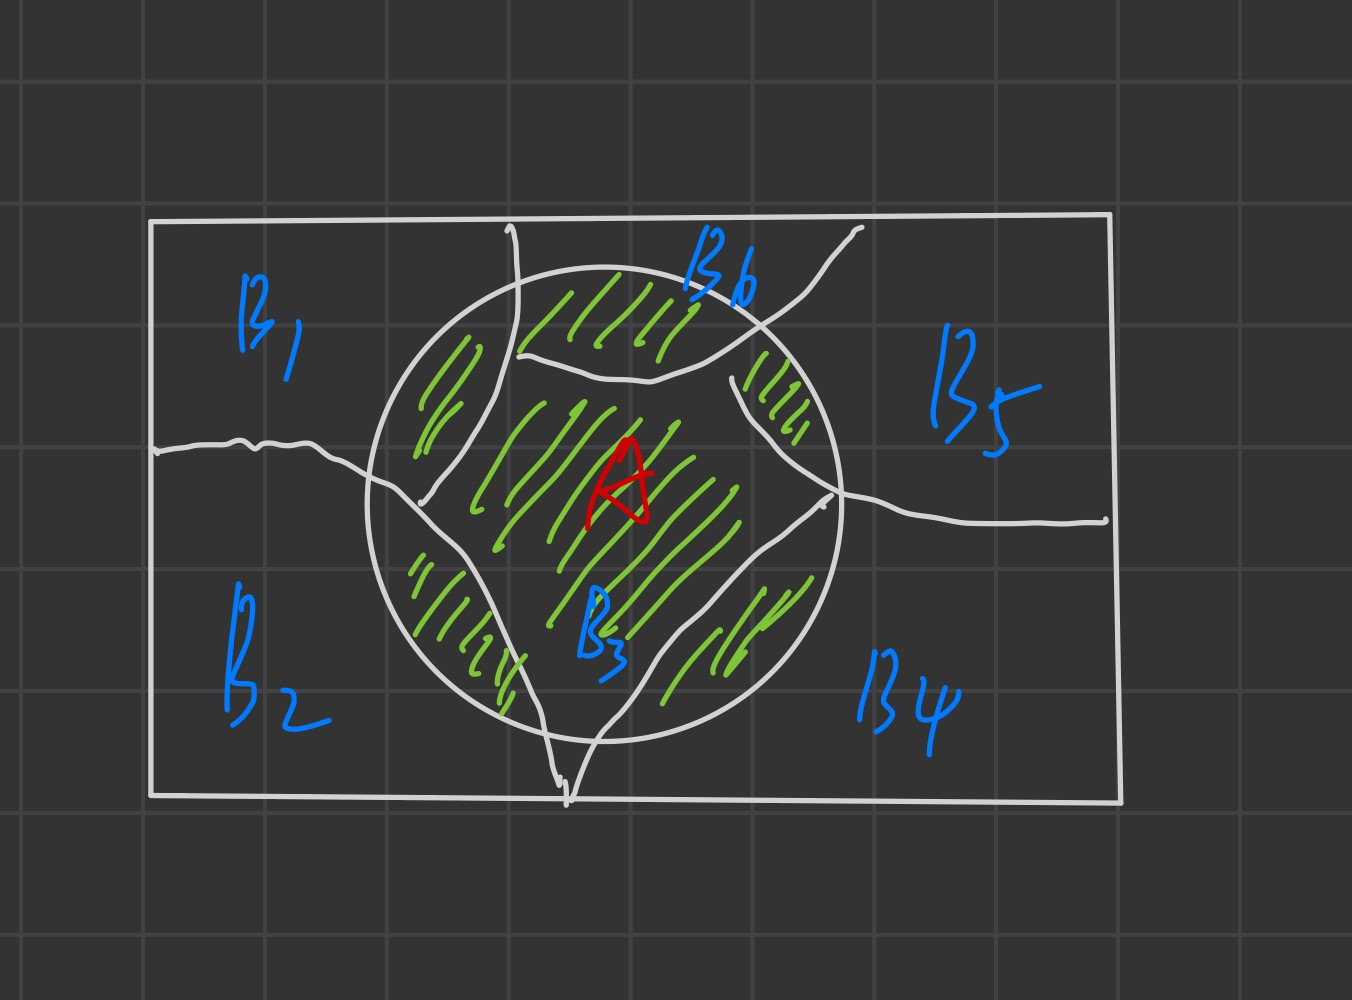
\includegraphics[width=5cm, height=4cm]{images/total_probability.jpg}
\end{center}
\end{annotation}

\begin{definition}
\rm {\color{red}贝叶斯公式} 设$B_1,B_2,\cdots,B_n$满足$\bigcup\limits_{i=1}^n B_i = \Omega$,$B_iB_j = \emptyset$且$P(A)>0, P(B_k) > 0,\; k=1,2,\cdots,n$,则
	$$
		P(B_j | A) = \frac{P(B_j)P(A|B_j)}{\sum\limits_{i=1}^n P(B_i)P(A|B_i)},\; j = 1,2,\cdots,n.
	$$
前提条件可以换成“若事件$A$能且只能与两两互不相容的事件$B_1,B_2,\cdots,B_n$之一同时发生”,这个条件实际上更有实际意义. 其中$P(B_i)$称为\redt{先验概率},条件概率$P(B_i | A)$称为\redt{后验概率}. 
\end{definition}

\begin{proof}
由于$P(A) > 0,P(B_k) > 0$,那么此时有
$$
P(B_kA) = P(A)P(B_k|A) = P(B_k)P(A|B_k). 
$$
故
$$
P(B_j|A) = \frac{P(B_j)P(A|B_j)}{P(A)}.
$$
在利用全概率公式即有
$$
P(B_j|A) = \frac{P(B_j)P(A|B_j)}{\sum\limits_{i =1}^n P(B_i)P(A|B_i)}.
$$
\end{proof}

\begin{annotation}
\rm 贝叶斯公式中先验概率$P(B_i)$反应了各种“原因”发生的可能的性大小,一般是以往的经验总结,在当前试验前就已经知道了. 若当前试验产生了事件$A$,这个信息将有助于探讨事件发生的原因. 后验概率$P(B_i|A)$它反映了试验之后对各种原因发生的可能性大小的新知识.
\end{annotation}

\begin{example}
\rm {\color{red}(贝叶斯决策)} 为了判定一个字母是"C"还是"O",通常采取抽取它的一个特征$X$. 然后再根据这个特征作出判决,这时贝叶斯决策常用的方法之一. 

以$A_1,A_2$分别表示被检验的字母为$C$或者$O$这一事件,它们的先验概率$P(A_1)$及$P(A_2)$应预先给定,此外要通过试验确定$P(X|A_1)$或者$P(X|A_2)$,由贝叶斯公式得
$$
P(A_i|X) = \frac{P(A_i)P(X|A_i)}{\sum\limits_{i=1}P(A_i)P(X|A_i)} 
$$
其中$i=1,2$. 若$P(A_1 | X) > P(A_2 | X)$,则做出决策,具有特征$X$的字母是$C$.
\end{example}

\begin{definition}
\rm 若事件$A,B$满足等式
$$
P(AB) = P(A)P(B),
$$
则称$A$与$B${\color{red}相互独立}. 
\end{definition}

\begin{annotation}
\rm {\color{blue} 从条件概率看两个事件的独立性,也就是其中一个发生的概率是不会影响另一个发生的概率}
\end{annotation}

\begin{corollary}
\rm 若事件$A$与$B$独立,则下列各对立事件也相互独立
$$
\{\overline{A}, B\},\, \{A,\overline{B}\}, \{\overline{A},\overline{B}\}
$$
\end{corollary}

\begin{proof}
由于
$$
\begin{array}{ll}
P(\overline{A}B) &= P(B-AB)=P(B)-P(AB)\\
&= P(B)-P(A)P(B) = P(B)[1-P(A)]\\
&= P(\overline{A})P(B).  
\end{array}
$$
同理可得$\{A,\overline{B}\}$. 特别因为$\overline{A}$和$B$独立,马上可以得到
$$
P(\overline{A}) = P(\overline{A}B \cup \bar{A}\bar{B}) = P(\overline{A})P(B) + P(\bar{A}\bar{B}). 
$$
移项即可得到$P(\bar{A}\bar{B}) = P(\overline{A})P(\overline{B})$. 
\end{proof}

\begin{definition}
\rm 推广至$n$个事件$A_1,\cdots,A_n$相互独立,需要$\binom n2 + \binom n3 + \cdots + \binom nn = 2^n - n -1$等式成立,即设任意的$1<k \leq n$,对任意$1 \leq i_1 \leq \cdots \leq i_k \leq n$满足等式
$$
P(A_{i_1}\cdots A_{i_k})=P(A_{i_1})\cdots P(A_{i_k}).
$$
\end{definition}

\begin{annotation}
\rm {\color{blue}任意事件两两独立并不能推出它们相互独立}.
\end{annotation}

\begin{proposition}
\rm 若$A,B$是两个相互独立的事件,则
$$
P(A-B) = P(A)P(\overline{B}).
$$
\end{proposition}

\begin{proof}
\rm 
$$
P(A-B) = P(A)-P(AB) = P(A)(1-P(B)) = P(A)P(\overline{B}).
$$
\end{proof}

\begin{proposition}
\rm 若$A_1,A_2,\cdots,A_n$是$n$个相互独立的事件,则
$$
P(A_1 \cup A_2 \cup \cdots \cup A_n) = 1-P(\overline{A}_1)P(\overline{A}_2)\cdots P(\overline{A}_n). 
$$
\end{proposition}

\begin{proof}
由于$\overline{A_1\cup A_2 \cup \cdots \cup A_n} = \overline{A}_1\overline{A}_2\cdots\overline{A}_n$,因此
$$
\begin{array}{ll}
P(A_1 \cup A_2 \cup \cdots \cup A_n) &= 1-P(\overline{A}_1\overline{A}_2\cdots\overline{A}_n)\\
&= 1 - P(\overline{A}_1)P(\overline{A}_2)\cdots P(\overline{A}_n).
\end{array}
$$
\end{proof}


\newpage
\section{随机变量及其概率分布}

\subsection{随机变量及其分部函数}

\begin{definition}
\rm 在样本空间$\Omega$上的实值函数$X=X(\omega),\, \omega \in \Omega$,称$X(\omega)$为{\color{red}随机变量},简记为$X$. $X$表示样本点到$\mathbb{R}$上一一映射.  
\end{definition}

\begin{annotation}
\rm 随机变量的概念引入是为了通过函数的image(实数)来描述preimage,即某一样本空间中的样本点, i.e. $P(X < 1)$. 随机变量是样本点的函数,因此在试验前我们只能知道它可能取那些值,而不确定它将取何值,这就是随机的含义. 
\begin{center}
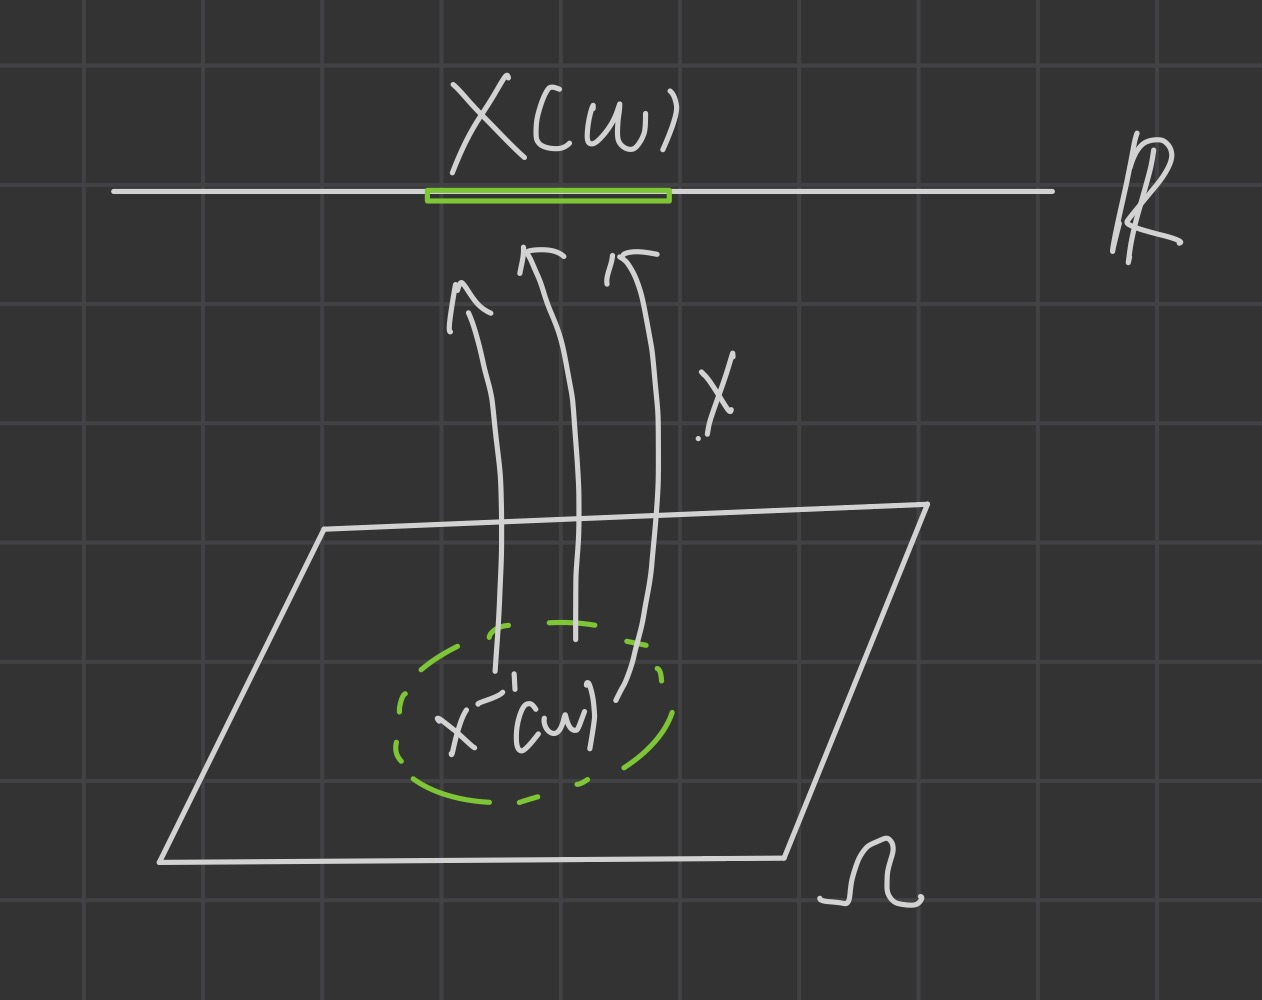
\includegraphics[width=5cm, height=4cm]{images/random_variable.jpg}
\end{center}
\end{annotation}

\begin{definition}
\rm 如果一个随机变量的可能取值是有限多个或者可数无穷多个,则称它为{\color{red}离散型随机变量}.
\end{definition}

\begin{annotation}
\rm 离散型随机变量可以理解为$\mathbb{R}$上的点.
\end{annotation}



\begin{definition}
\rm 设离散型随机变量$X$的可能取值是$x_k(k=1,2,\cdots)$,$X$取各可能值的概率为
$$
P\{X=x_k\} = p_k, k=1,2,\cdots,
$$
称上式为离散型随机变量$X$的\redt{概率(质量)分布}(probability mass function)或者分部律,其中$P$是一个概率函数.
\end{definition}

\begin{proposition}
\rm 分部律充要条件
\begin{enumerate}
	\item $p_k \geq 0,k=1,2,\cdots$;
	\item $\sum\limits_{k=1}^\infty p_k = 1$.
\end{enumerate}
\end{proposition}

\begin{proof}
{\color{red}(2)} $1 = P[\bigcup\limits_{k=1}^{\infty}\{X= x_k\}] = \sum\limits_{k=1}^{\infty} P\{X=x_k\}$,这里说明了$\{X=x_i\} \cap \{X = x_j\} = \emptyset, i \neq j$.
\end{proof}

\begin{definition}
\rm 设$X$是一个随机变量,对于任意实数$x$,函数
$$
F(x) = P\{X \leq x\},\,-\infty < x < +\infty,
$$
称为随机变量$X$的\redt{分布函数}(累积分布函数或者cumulative distribution function). 
\end{definition}

\begin{proposition}
\rm {\color{red} 分布函数的本质意义} 给定随机变量$X$的分布函数$F(x)$,则对任意的$x_1 < x_2$,有
$$
P\{x_1 < X \leq x_2\} = F(x_2) - F(x_1).
$$
\end{proposition}

\begin{proof}
$$
P\{x_1 < X \leq x_2\} = P(X \leq x_2) - P(X \leq x_1) = F(x_2)-F(x_1).
$$
\end{proof}

\begin{annotation}
\rm {\color{blue}从上式的证明中我们知道只要对一切实数$x$给出了概率$P\{X \leq x\}$,就能算出$X$落入某个区间$(a,b]$的概率,特别地再利用概率的性质还可以算出$X$属于$\mathbb{R}$上某些相当复杂的点集}. 为了计算概率,必要要求随机变量具有可测性,而分布函数的引进则把对于随机变量的概率计算转换为了对分布函数的数值运算. 
\end{annotation}

\begin{proposition}
\rm 分布函数性质如下
\begin{enumerate}
	\item $F(x)$是非减函数,即当$x_1 < x_2$时,$F(x_1) \leq F(x_2)$ ({\color{red}分部函数充要条件之一});
	\item $0 \leq F(x) \leq 1$; $\lim\limits_{x \rightarrow -\infty}F(x) =F(-\infty) = 0$; $\lim\limits_{x \rightarrow +\infty}F(x) =F(+\infty)= 1$ ({\color{red}分部函数充要条件之一});
	\item $F(x)$是右连续的,即$F(x+0) = F(x)$ ({\color{red}分部函数充要条件之一}); 
	\item 对任意的$x$,有$P\{X = x\} = F(x) - F(x-0)$;  
\end{enumerate}
\end{proposition}

\begin{proof}
\rm  
{\color{red}(1)} 若$x_2 > x_1$,则
$$
F(x_2)-F(x_1) = P\{x_1 < X \leq x_2\} \geq 0.
$$ 

{\color{red}(2)} 因
$$
\begin{array}{ll}
P\{-\infty < X < +\infty\} &= \sum\limits_{n=-\infty}^{+\infty}P\{n \leq X \leq n+1\} \\ 
&= \sum\limits_{n=-\infty}^{+\infty}\left[F(n+1)-F(n)\right]\\
&= \lim\limits_{n \rightarrow +\infty}F(n) - \lim\limits_{m \to -\infty} F(m)= 1 
\end{array}.
$$
上面只是说明了有理数趋于无穷的极限,需要推广任意实数上. 因为$F(x)$的单调性($ F(\lfloor x \rfloor) \leq F(x) \leq F(\lceil x \rceil)$),所以$\lim\limits_{x \rightarrow -\infty}F(x) = \lim\limits_{m \to -\infty} F(m)$,$\lim\limits_{x \rightarrow +\infty}F(x)= \lim\limits_{n \rightarrow +\infty}F(n)$存在. 因为$0\leq F(x) \leq 1$,故
$$
\lim\limits_{x \rightarrow -\infty}F(x) =0 , \lim\limits_{x \rightarrow +\infty}F(x)=1.
$$


{\color{red}(3)} 从(1)(2)可知$F(x)$是单调有界的,若存在间断点,那么只能是第一类间断点,即$F(x)$的任意一点$x_0$处的右极限$F(x_0+0)$是存在的,实际也可以从单调有界来看出从$x_0$右边趋于$x_0$时候$F(x)$极限存在. 现在来证明$F(x+0) = F(x)$. 这里可取一个单调减的数列$x_1 > x_2 > \cdots > x_n > \cdots> x_0$, 即证$\lim\limits_{n \rightarrow \infty} F(x_n) = F(x_0)$. 而
$$
\begin{array}{ll}
F(x_1) - F(x_0) =  P\{x_0 < X \leq x_1\} =  P\left[\bigcup\limits_{i=1}^\infty\{x_{i+1} < X \leq x_{i}\}\right] = \sum\limits_{i=1}^\infty P\{x_{i+1} < X \leq x_i\} \\
= \sum\limits_{i=1}^\infty \left[F(x_i) - F(x_{i+1})\right] =  F(x_1) - \lim\limits_{i \to \infty} F(x_{i+1}),
\end{array}
$$
因此有$F(x_0) = \lim\limits_{i \to \infty} F(x_{i+1}) = F(x_0+0)$. 注意第二个等号使用了一个重要的极限
$$
\{x_0 < X \leq x_1\} = \lim\limits_{n \rightarrow \infty}\bigcup\limits_{i=1}^n\{x_{i+1} < X \leq x_{i}\}
$$

这里我们可以用\ref{probability-axiom: lemma1}来证,我们让$A_n = \{X \leq x_0 + x_n\}$,其中$x_n$是一个单调递减的极限为$0$数列. 于是
$$
P(\lim\limits_{n \to \infty}A_n) = P\{X \leq x_0\} =  F(x_0) = \lim\limits_{n \to \infty} P(A_n) = \lim\limits_{n\to \infty}F(x_0+x_n) = F(x_0 + 0). 
$$

{\color{red}(4)} 这里因为无法保证是右连续的,所以减去$x$除的右极限的跃度就是这$x$这一点的概率.
\end{proof}

\begin{proposition}
\rm 特殊点和区间的概率分布
$$
\begin{array}{ll}
P\{X = x\} = F(x)-F(x-0) \\
P\{X < x\} = F(x-0) \\
P\{X > x\} = 1-F(x) \\
P\{X \geq x\} = 1-F(x-0) 
\end{array} 
$$
\end{proposition}

\begin{annotation}
\rm {\color{red}上述更贴切的说明了分别函数是一种分析性质良好的函数,给定了分布函数就能计算处各种事件的概率}. 
\end{annotation}

\begin{proposition}
\rm 给定离散型随机变量的分布律$P\{X=x_i\}=p_i,i = 1,2,\cdots$,它的分布函数$F(x)$为
$$
F(x) = P\{X < x\} = \sum\limits_{x_k < x}p(x_k)
$$
\end{proposition}


\begin{definition}
\rm 如果对随机变量$X$的分布函数$F(x)$,存在一个非负可积函数$f(x)$,使得对任意的实数$x$,都有
$$
F(x) = \int_{-\infty}^x f(t)dt, - \infty < x < + \infty,
$$
那么称$X$为{\color{red}连续型随机变量},函数$f(x)$称为$X$的{\color{red}概率密度}. 
\end{definition}

\begin{annotation}
\rm 连续随机变量可以理解为$\mathbb{R}$上的区间. 自然地,事件运算对应了区间集合运算. 
\end{annotation}

\begin{proposition}
\rm 连续型随机变量的分布函数$F(x)$是在$(-\infty,+\infty)$上连续的.
\end{proposition}

\begin{proposition}\label{probability-density-func: prop1}
\rm 概率密度函数$f(x)$的性质如下
\begin{enumerate}
	\item $f(x) \geq 0$ ({\color{red}$f(x)$是概率密度函数的充要条件之一});
	\item 对于任意实数$x$,有$P\{X=x\} = F(x)-F(x-0) = 0$.
	\item $F(+\infty) = \int_{-\infty}^{+\infty} f(t)dt = 1$ ({\color{red}$f(x)$是概率密度函数的充要条件之一});
	\item 对任意实数$x_1 < x_2$,有$P\{x_1 < X \leq x_2 \} = F(x_2)-F(x_1) = \int_{x_1}^{x_2} f(t)dt$;
	\item 在$f(x)$的连续点处有$F'(x) = f(x)$. (证明见高数积分上限函数一节) 
\end{enumerate}
\end{proposition}

\begin{proof}
证明见高数积分上限函数一节
\end{proof}

\begin{annotation}
\rm {\color{blue}上述性质表明,一个事件的概率为0,这件事并不一定是不可能事件; 同样地,一个事件概率等于1,这件事也不一定是必然事件}. 
\end{annotation}

\begin{proposition}
\rm 若$X$是连续型随机变量,则
$$
P\{x_1 < X \leq x_2\} = P\{x_1 \leq X  < x_2\} = P\{x_1 < X < x_2\} = P\{x_1 \leq  X \leq x_2\}.
$$
\end{proposition}

\begin{proof}
由proposition \ref{probability-density-func: prop1}中(2)易得. 
\end{proof}


\subsection{常用分布}

\begin{definition}
\rm 若随机变量$X$只取常数$c$,即$P\{X=c\} = 1$,那么这时的分布函数为
$$
F(x) = \left\{\begin{array}{ll}
1, &x \geq c \\
0, &x < c
\end{array} \right. .
$$
则称$X$服从\redt{退化分布},又称\redt{单点分布}. 
\end{definition}

\begin{definition}
\rm 如果随机变量$X$的分布律为
$$
\begin{array}{c|cc}
X & 0 & 1\\
\hline
P & 1-p & p
\end{array}
$$
其中$0 < p < 1$,则称$X$服从参数为$p$的\redt{$0 - 1$分布}或者\redt{两点分布}.
\end{definition}

\begin{definition}
\rm 如果随机变量$X$的分布律为
$$
P\{X = k\} = C_n^kp^kq^{n-k}, k = 0,1,2,\cdots,n,
$$
其中$0 < p < 1, q= 1- p$,则称$X$服从参数为$n,p$的\redt{二项分布},记做$X \sim B(n,p)$.
\end{definition}

\begin{annotation}
\rm 在$n$重伯努利试验中,若每次试验成功率为$p(0 < p < 1)$,则在$n$次独立重复试验中成功的总次数$X$服从二项分布.
\end{annotation}

\begin{proposition}
\rm \redt{二项分布分析性质} 若$X \sim B(n,p)$,当$n$固定时,$P\{X=k\}$先随$k$增加而增大,达到某一极值后又逐渐下降,其在$k=\lfloor(n+1)p\rfloor$取得极值. 
\end{proposition}

\begin{proof}
\rm 我们来考察
$$
\frac{P\{X=k\}}{P\{X=k-1\}} = \frac{C_n^k p}{C_n^{k-1}q} = \frac{(n+1-k)p}{kq} = \frac{(n+1)p-(1-q)k}{kq} = 1+ \frac{(n+1)p - k}{kq}
$$
因此

当$k < (n+1)p$时,$P\{X=k\} > P\{X = k-1\}$;

当$k = (n+1)p$时,$P\{X=k\} = P\{X = k-1\}$;

当$k > (n+1)p$时,$P\{X=k\} < P\{X = k-1\}$;

因为$(n+1)p$不一定是整数,所以存在整数$m$,使得$(n+1)p-1 < m \leq (n+1)p$,即当$k = m$时$P\{X=k\}$达到最大值.  
\end{proof}

\begin{definition}
\rm 如果随机变量$X$的分布律为
$$
P\{X=k\} = pq^{k-1}, k =1,2,\cdots,
$$
其中$0 < p < 1, q= 1- p$,则称$X$服从参数为$p$的\redt{几何分布},或称$X$具有几何分布.
\end{definition}

\begin{annotation}
\rm 在独立地重复做一系列伯努利试验中,若每次试验成功率为$p(0 < p < 1)$,则在第$k$次试验时才首次试验成功的概率服从几何分布.
\end{annotation}

\begin{proposition}
\rm \redt{几何分布具有无记忆性},即若假定前$m$次没有成功,设随机变量$X'$为为了达到首次成功还需要做的试验数,则$X'$依然服从几何分布.
\end{proposition}

\begin{proof}
$$
\begin{array}{ll}
P\{X' = k\} = P\{X=m+k| X > m\} = \frac{P\{X = m+k\}}{P\{X > m\}} = \frac{pq^{m+k-1}}{q^m} = pq^{k-1}. 
\end{array}
$$
\end{proof}

\begin{definition}
\rm 若随机变量$X$的分布律为
$$
P\{X=k\} = C_{k-1}^{r-1}p^rq^{k-r},k=r,r+1,\cdots,
$$
其中$r \geq 1$,则称$X$服从\redt{巴斯卡分布}. 特别地当$r=1$时,就是几何分布. 
\end{definition}

\begin{annotation}
\rm 在独立地重复做一系列伯努利试验中,若每次试验成功率为$p(0 < p < 1)$,那么第$r$次成功时的试验次数的概率服从巴斯卡分布. 若考虑第$r$次成功时的失败试验次数的概率,即
$$
P\{X = k\} = \binom{r+k-1}{r-1}p^{r}q^{k}.
$$
上述概率分布被称为\redt{负二项分布},其中的组合数项可以写作
$$
(-1)^{k}{\frac {(-r)(-r-1)(-r-2)\dotsm (-r-k+1)}{k!}}=(-1)^{k}{\binom {-r}{k}},
$$
那么原式就为
$$
P\{X = k\} = \binom {-r}{k} p^r(-q)^k. 
$$
这就是"负"字的来源. 
\end{annotation}

\begin{definition}
\rm 如果随机变量$X$的分布律为
$$
P\{X=k\} = \frac{C_M^kC_{N-M}^{n-k}}{C_{N}^n}, k=l_1,\cdots,l_2,
$$
其中$l_1 = \max(0,n-N+M), l_2 = \min(M,n)$,则称随机变量$X$服从参数$n,N,M$的\redt{超几何分布}.
\end{definition}

\begin{annotation}
\rm 如果$N$件产品中含有$M$件次品,从中任意一次取出$n$件,令$X=$抽取的$n$件产品中的次品件数,则$X$服从参数$n,N,M$的\redt{超几何分布}. 
\end{annotation}

\begin{definition}
\rm 如果随机变量$X$的分布律为
$$
P\{X=k\} = \frac{\lambda^k}{k!}e^{-\lambda}, k = 0,1,2,\cdots,
$$
其中$\lambda > 0$为常数,则称随机变量$X$服从参数为$\lambda$的\redt{泊松分布},记为$X \sim P(\lambda)$. 
\end{definition}

\begin{annotation}
\rm 
$$
\sum\limits_{k=0}^{\infty} P\{X =k\} = \sum\limits_{k=0}^{\infty}\frac{\lambda^k}{k!}e^{-\lambda} = e^{-\lambda}\sum\limits_{k=0}^{\infty}\frac{\lambda^k}{k!} = e^{-\lambda}e^{\lambda} = 1,
$$
其中$e^x = \sum\limits_{k=0}^{\infty}\frac{\lambda^k}{k!}$.
\end{annotation}

\begin{theorem}
\rm {\color{red} 泊松定理} 设$\lambda > 0$是一个常数,$n$是任意整数,设$np_n = \lambda$,则对于任一固定的非负整数$k$,有
$$
\lim\limits_{n \rightarrow \infty}C_n^kp_n^k(1-p_n)^{n-k} = \frac{\lambda^ke^{-\lambda}}{k!}.
$$
\end{theorem}

\begin{annotation}
\rm 应用泊松定理来做二项式近似计算要求$n$较大,$p$较少,并且$np$大小适中,则
$$
C_n^kp^k(1-p)^{n-k} \approx \frac{\lambda^ke^{-\lambda}}{k!},
$$
其中$\lambda = np$.
\end{annotation}

\begin{proposition}
\rm 若我们关注的随机变量$X$是表示某个事件$A$发生的次数$k$且$X\sim P(\lambda)$,假定它具有有下面三个性质
\begin{enumerate}
	\item {\color{red}平稳性} 在$[t_0,t_0+t)$中$A$发生个数只与时间间隔长度有关而与时间起点$t_0$无关. 若以$P_k(t)$表示在长度为$t$的时间区间中$A$发生的$k$次的概率,那么对任意的$t$有
	$$
	\sum\limits_{k=0}^{\infty} P_k(t) = 1
	$$
	成立. 过程的平稳性表示了它的概率规律不随时间的推移而改变.
	\item {\color{red}独立增量性(无后效性)} 在$[t_0,t_0+t)$中$A$发生的$k$次这一事件与时刻$t_0$以前发生的事件独立. 独立增量性表明在互不相交的时间区间内过程进行的相互独立性.
	\item {\color{red}普通性} 在充分小的时间间隔内,$A$最多发生一次. 即,若记
	$$
	\psi(t) = \sum\limits_{k=2}^{\infty} P_k(t) = 1-P_0(t)-P_1(t),
	$$
	那么有
	$$
	\lim\limits_{t \rightarrow 0} \frac{\psi(t)}{t} = 0.
	$$
	换句话说,就是在同一时间瞬时$A$不可能发生$2$次以上. 由上述条件求出来的$P_k(t)$固定$t$就是泊松分布. 
\end{enumerate}
\end{proposition}

\begin{definition}
\rm 如果连续型随机变量$X$的概率密度为
$$
f(x) = \left\{\begin{array}{ll}
\frac{1}{b-a} & a \leq x \leq b\\
0 & \text{other}
\end{array}\right.,
$$
则称$X$在区间$[a,b]$上服从\redt{均匀分布},记做$X \sim U[a,b]$. 其的分布函数为
$$
F(x) = \left\{\begin{array}{ll}
0 & x < a \\
\frac{x-a}{b-a} & a \leq x < b\\
1 & x \geq b
\end{array}\right..
$$
\end{definition}

\begin{proposition}
\rm 设$X \sim U[a,b]$,则对$a \leq c < d \leq b$,有
$$
P\{c\leq x \leq d\} = \frac{d-c}{b-a}.
$$
\end{proposition}

%https://en.wikipedia.org/wiki/Exponential_distribution
\begin{definition}
\rm 如果连续型随机变量$X$的概率密度为
$$
f(x) = \left\{ \begin{array}{ll}
\lambda e^{-\lambda x} & x > 0 \\
0 & x \leq 0
\end{array}\right.,
$$
其中$\lambda > 0$是个常数,则称$X$服从参数为$\lambda$的\redt{指数分布},记做$X \sim E(\lambda)$. 其分布函数为
$$
F(x) = \left\{\begin{array}{ll}
1 - e^{-\lambda x} & x > 0 \\
0 & x \leq 0
\end{array}\right..
$$
\end{definition}

\begin{proposition}
\rm 设$X \sim E(\lambda)$,则有
\begin{enumerate}
	\item 当$t > 0$时,$P\{X > t\} = \int_t^{+\infty} \lambda e^{-\lambda t}dt$;
	\item 当$t > 0, s >0$时,$P\{X > t+s |x > s\} = \frac{P\{X > t+s \}}{P\{X > s\}} = \frac{e^{-\lambda(t+s)}}{e^{-\lambda}(s)} =1- e^{-\lambda t} = P\{X > t\}$. 此性质称为指数分布具有"无记忆性". 
\end{enumerate}
\end{proposition}

\begin{definition}
\rm 如果连续性随机变量的概率密度为
$$
f(x) = \frac{1}{\sqrt{2\pi}\sigma}e^{-\frac{(x-\mu)^2}{2\sigma^2}},
$$
其中$\mu,\sigma$为常数且$\sigma > 0$,则称$X$服从参数为$\mu,\sigma$的\redt{正态分布},记做$X~N(\mu,\sigma^2)$. 当$\mu=0,\sigma^2 =1$时,即$X \sim N(0,1)$,称$X$服从\redt{标准正态分布},此时用$\varphi(x)$表示$X$的概率密度,即
$$
\varphi(x) = \frac{1}{\sqrt{2\pi}}e^{-\frac{x^2}{2}}.
$$
当$X \sim N(\mu,\sigma^2)$,其分布函数为
$$
F(x) = \frac{1}{\sqrt{2\pi}\sigma}\int_{-\infty}^{x}e^{-\frac{(t-\mu)^2}{2\sigma^2}}dt. 
$$
当$X~N(0,1)$,其分布函数为
$$
\Phi(x) = \frac{1}{\sqrt{2\pi}}\int_{-\infty}^x e^{-\frac{t^2}{2}}dt.
$$
\end{definition}

\begin{annotation}
\rm \redt{正态分布的图像性质} 正态分布概率密度图像是关于$x = \mu$对称的. 当$\sigma$越小时,分布越集中在$x=a$附近; $\sigma$越大时,分布就越平坦. 若$X$服从$N(\mu,\sigma^2)$,在一次试验中$X$几乎都落在$(\mu-3\sigma,\mu + 3\sigma)$.
\end{annotation}

\begin{proposition}
\rm \redt{正态分布到标准正态分布的转换} 设$X \sim N(\mu,\sigma^2)$,则$Z = \frac{X-\mu}{\sigma} \sim N(0,1)$. 
\end{proposition}

\begin{proof}
\rm $Z=\frac{X-\mu}{\sigma}$的分布函数为
$$
P\{Z \leq x\} = P\{\frac{X-\mu}{\sigma} \leq x\} = P\{X \leq \mu + \sigma x\} =  \frac{1}{\sqrt{2\pi}\sigma}\int_{-\infty}^{\mu+\sigma x}e^{-\frac{(t-\mu)^2}{2\sigma^2}}dt.
$$
令$u = \frac{t-\mu}{\sigma}$,那么$t = \sigma u + \mu$,于是
$$
P\{Z \leq x\} = \frac{1}{\sqrt{2\pi}}\int_{-\infty}^{x} e^{-\frac{u^2}{2}}du = \Phi(x). 
$$
由此$Z \sim N(0,1)$.
\end{proof}

\begin{corollary}
\rm 若$X \sim N(\mu,\sigma^2)$,则其分布函数$F(x)$可写成
$$
F(x) = P\{X \leq x \} = P\{ \frac{X-\mu}{\sigma} \leq \frac{x-\mu}{\sigma} \} = \Phi(\frac{x-\mu}{\sigma}). 
$$
\end{corollary}

\begin{proposition}
\rm 设$X \sim N(\mu,\sigma^2)$,其分布函数为$F(x)$,则
\begin{enumerate}
	\item $P\{a < x \leq b\} = \Phi(\frac{b-\mu}{\sigma}) - \Phi(\frac{a-\mu}{\sigma})$;
	\item 概率函数$f(x)$关于$x=\mu$对称,$\varphi(x)$是偶函数;
	\item $\Phi(-x) = 1-\Phi(x)$,$\Phi(0) = \frac{1}{2}$;
	\item 当$X \sim N(0,1)$且$a > 0$时,$P\{|X| \leq a\} = 1-2\Phi(-a) = 2\Phi(a) - 1$. 
\end{enumerate}
\end{proposition}

\begin{proof}
{\color{red}(4)}
$$
I(a)=\int_0^{\infty}e^{-ax^2}dx =\frac12 \sqrt{\frac{\pi}{a}}
$$
\end{proof}

\begin{definition}
\rm 如果连续型随机变量$X$的概率密度为
$$
f(x) = \left\{ \begin{array}{ll}
\frac{\beta^\alpha}{\Gamma(\alpha)}x^{\alpha-1}e^{-\beta x} &  x > 0 \\
0 & x \leq 0 
\end{array} \right.
$$
其中$\alpha,\beta$,则称$X$服从\redt{伽马分布},记为$X \sim \Gamma(\alpha,\beta)$.
\end{definition}

\begin{annotation}
\rm 由伽马函数
$$
\Gamma(\alpha) = \int_{0}^{+\infty} x^{\alpha-1}e^{-x}dx.
$$
令$x = \beta t$,那么则有
$$
\Gamma(\alpha,\beta) = \beta^\alpha \int_{0}^{+\infty} t^{\alpha-1} e^{-\beta t} dt. 
$$
因此
$$
\frac{\beta^\alpha}{\Gamma(\alpha,\beta)}\int_{0}^{+\infty} t^{\alpha-1} e^{-\beta t} dt = 1. 
$$
\end{annotation}

\begin{proposition}
\rm 设$X \sim \Gamma(\alpha,\beta)$,则下面性质成立
\begin{enumerate}
	\item $\Gamma(1,\beta) \sim E(\beta)$;
	\item $\Gamma(\alpha,1)$叫做标准伽马分布;
\end{enumerate}
\end{proposition}

\begin{proposition}\label{gamma-distribution-additivity}
\rm \redt{$\Gamma$分布的可加性} 设随机变量$X_1,X_2,\cdots,X_n$相互独立,且$X_i \sim \Gamma(\alpha_i,\beta),i=1,\cdots,n$,则
$$
\sum\limits_{i=1}^n X_i \sim \Gamma(\sum\limits_{i=1}^n \alpha_i,\beta).
$$
\end{proposition}

\begin{proof}

\end{proof}

\subsection{随机变量的函数的分布}
\begin{annotation}
\rm ??? CDF的导数是否等于PDF?
$$
F(x)' = f(x)
$$
\end{annotation}

\begin{definition}
\rm $y=f(x)$实际上是一个可测函数. 
\end{definition}

\begin{annotation}
\rm 若随机变量$X$为离散型变量,把$Y=g(X)$可以取的不同值找出来,把与某个值相应的全部$X$值的概率加起来,即得$Y$取这个值的概率.
\end{annotation}

\begin{annotation}
\rm 若随机变量$Y$为连续性变量,把$Y=g(x)$可以取的不同值找出来,对应某个$y$值而言,求$F(y) = P\{Y \leq y\}$,就是把对应全部的$X$的概率积出来,即
$$
\int\limits_{g(x) \leq y} f_X(t)dt.
$$
注意其中$f_(X)$可能是分段函数,对不同范围的$x$要分别积分再加起来. 
\end{annotation}

\begin{theorem}
\rm 设随机变量$X$具有概率密度$f_X(x)$对任意实数都有定义. 若给定$g(x)$是严格单调的,其反函数$g^{-1}(x)$有\redt{连续导数}(有可能怕破坏$f_X(x)$的连续性?). 则$Y = g(X)$是连续型随机变量,其概率密度为
$$
f_Y(y) = \left\{ \begin{array}{ll}
f_X\left[ g^{-1}(y) \right]|\left[g^{-1}(y)\right]'| & \alpha < y < \beta \\
0 , & \text{otherwise}
\end{array}\right. ,
$$
其中$\alpha = \min(g(-\infty), g(+\infty)),\beta = \max(g(-\infty), g(+\infty))$. 
\end{theorem}

\begin{proof}
若$g(x)$是严格单调增大,且其反函数$g^{-1}(x)$是有连续导数. 给定任意实数$y \in (\alpha,\beta)$,那么
$$
F_Y(y) = P\{Y \leq y \} = P\{X \leq g^{-1}(y)\} = F_X(g^{-1}(y))
$$
对$F_Y(y)$关于$y$求导,即有$f_Y(y) = f_X\left[ g^{-1}(y) \right]\left[g^{-1}(y)\right]'$. 若给定实数$y \leq \alpha$,那么显然有$F_Y(a) = 0$; 当$y \geq \beta$,有$F_Y(a) = 1$.

同理若$g(x)$是严格单调递减,若给定任意实数$y \in (\alpha,\beta)$,那么
$$
F_Y(y) = P\{Y \leq y \} = P\{X \geq g^{-1}(y)\} = 1-F_Y(g^{-1}(y)), 
$$
对$F_Y(y)$关于$y$求导,即有$f_Y(y) = -f_X\left[ g^{-1}(y) \right]\left[g^{-1}(y)\right]'$,当$g(x)$是严格单调递减时,$g^{-1}(y)$也是严格单调递减的,因此$\left[g^{-1}(y)\right]' < 0$,所以这里有$f_X\left[ g^{-1}(y) \right]|\left[g^{-1}(y)\right]'|$. 综合两式便得命题中的概率密度函数. 
\end{proof}

\begin{corollary}
\rm 设随机变量$X$具有概率密度$f_X(x)$对任意实数都有定义. 若$g(x)$在不相互重叠的区间$I_1,I_2,\cdots$上逐段严格单调,其反函数分别为$h_1(y),h_2(y),\cdots$,而且$h_1'(y),h_2'(y),\cdots$均为连续函数. 则$Y=g(X)$是连续型随机变量,其概率密度为
$$
f_Y(y) = \sum\limits_{i}f_X\left[h_i(y)\right]|h_i'(y)|. 
$$
\end{corollary}

\begin{corollary}
\rm 随机变量$X$的概率密度$f(x)$,则$Y=X+b$的密度函数为$f(y-b)$.
\end{corollary}

\subsection{常见随机变量的函数分布}

\begin{example}
\rm 若$X \sim N(\sigma^2,\mu)$,$Y=aX+b,a\neq 0$. 

那么$g^{-1}(y) = \frac{y-b}{a}$,则$Y$的密度函数为
$$
f_y(y) = f_x[g^{-1}(y)]|[g^{-1}(y)]'|= \frac{f_x(\frac{y-b}{a})}{|a|} = \frac{1}{\sqrt{2\pi}\sigma|a|}e^{-\frac{(\frac{y-b}{a}-\mu)^2}{2\sigma^2}} = \frac{1}{\sqrt{2\pi}\sigma|a|}e^{-\frac{(y-(b+a\mu))^2}{2\sigma^2a^2}}.
$$
因此$y \sim N(a\mu+b,a^2\sigma^2)$.
\end{example}

\begin{example}
\rm 若$Y=X^2$.

因$Y \geq 0$,那么$P\{Y \leq 0\} = 0$. 当$y > 0$时,则有
$$
P\{Y \leq y\} = P\{X^2 \leq y\} = P\{-\sqrt{Y} \leq X \leq -\sqrt{Y}\} = \int_{-\sqrt{y}}^{\sqrt{y}} f(t)dt.
$$
对$y$求导数,得$Y$的密度函数为
$$
f_y(y) = [F_x(\sqrt{y})-F_x(-\sqrt{y})]' = \frac{1}{2\sqrt{y}}[f(\sqrt{y}) + f(-\sqrt{y})].
$$
当$y \leq 0$时,$f_y(y)=0$. 
\end{example}

\begin{example}\label{normal-distribution-square}
\rm 若$X \sim N(0,1)$,求$Y=X^2$.

那么在$y > 0$时,有
$$
f_y(y) = \frac{1}{2\sqrt{y}}\left[ \frac{1}{\sqrt{2\pi}} e^{-\frac{y}{2}} + \frac{1}{\sqrt{2\pi}} e^{-\frac{y}{2}} \right] = \frac{1}{\sqrt{2\pi}}y^{-\frac{1}{2}}e^{-\frac{y}{2}}. 
$$
在$y=0$,有$f_y(y) = 0$. \bluet{这里有$Y \sim \Gamma(\frac{1}{2},\frac{1}{2})$}.
\end{example}


\newpage
\section{多维随机变量及其分布}

\subsection{多维分布}
\begin{definition}
\rm 若随机变量$X_1(\omega),X_2(\omega),\cdots,X_n(\omega)$定义在同一概率空间$(\Omega,\mathscr{F},P)$上,则称
$$
X(\omega) = (X_1(\omega),X_2(\omega),\cdots,X_n(\omega))
$$
构成一个\redt{$n$维随机向量},亦称\redt{$n$维随机变量}.
\end{definition}

\begin{annotation}
\rm 等待些许感受
\begin{center}
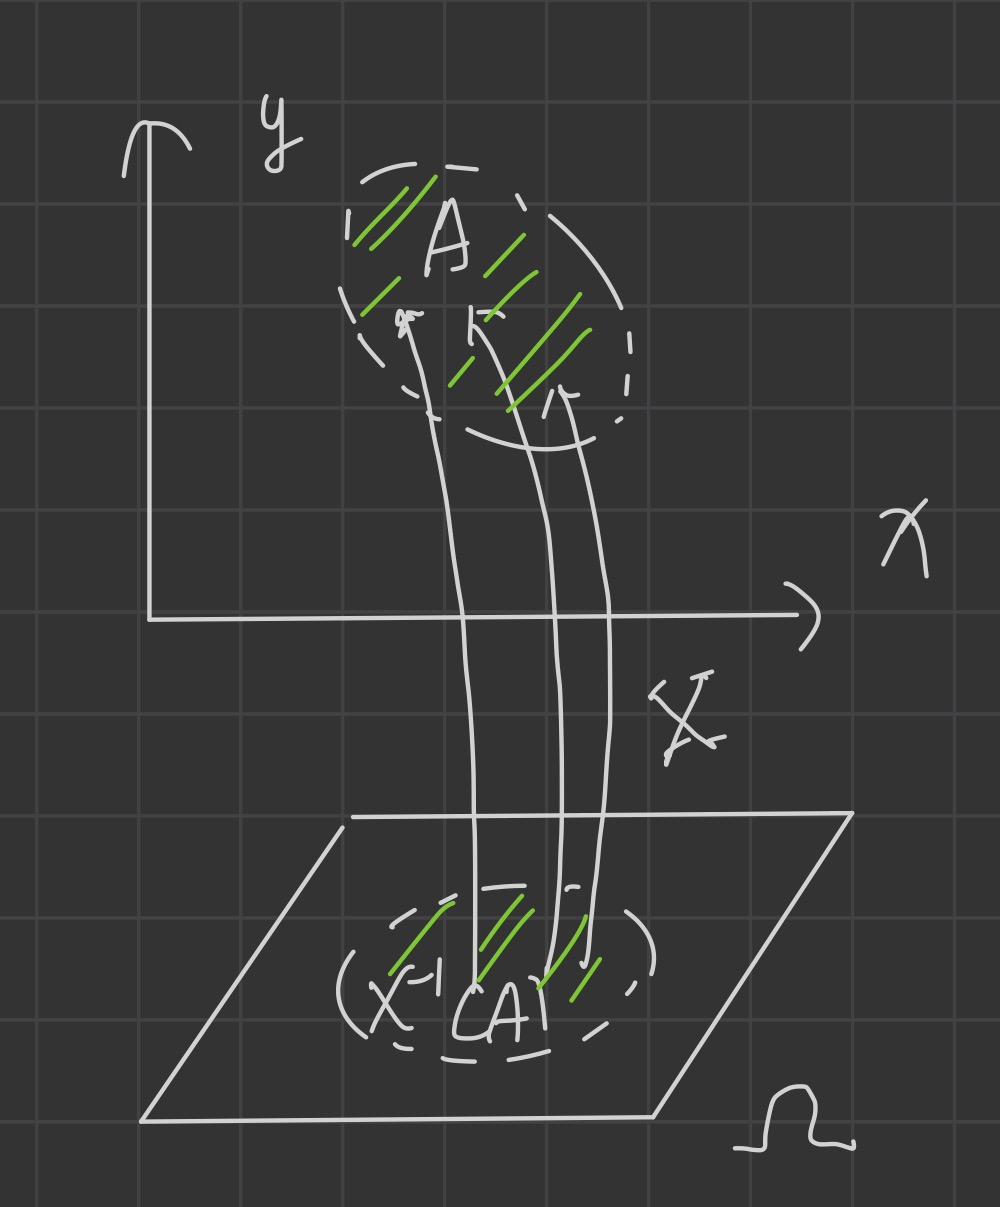
\includegraphics[width=5cm, height=4cm]{images/random_vector.jpg}
\end{center}
\end{annotation}

\begin{definition}
\rm 称$n$元函数
$$
F(x_1,x_2,\cdots,x_n) = P(X_1 \leq x_1, X_2 \leq x_2,\cdots, X_n \leq x_n)
$$
为$n$维随机变量$X=(X_1,X_2,\cdots,X_n)$的\redt{(联合)分布函数}. 
\end{definition}

\begin{proposition}
\rm 多元分布函数的基本性质
\begin{enumerate}
	\item 关于每个变元是单调不减;
	\item $0 \leq F(x_1,x_2,\cdots,x_n) \leq 1$;
	\item $F(x_1,x_2,\cdots,-\infty,\cdots,x_n) = 0,F(+\infty,+\infty,\cdots,+\infty) = 1$;
	\item 关于每个变元右连续;
	\item 对任意$x_1 < x_2, y_1 < y_2$,都有
	$$
	F(x_2,y_2)-F(x_1,y_2) - F(x_2,y_1) + F(x_1,y_1) \geq 0.
	$$
	上述实际上就是概率$P\{x_1 < X \leq X_2, y_1 < Y \leq y_2\}$.
\end{enumerate}
\end{proposition}


\begin{definition}
\rm 如果每一个$X_i$都是一个离散型随机变量,$i = 1,\cdots, n$,则称
$X = (X_1,\cdots, X_n)$为一$n$维离散随机变量. 设$X_i$的所有
可能取值 (有限或可数个) 为$\{a_{i1}, a_{i2}, \cdots \}, i = 1,\cdots, n$,则称
$$
p(j_1,j_2,\cdots,j_n) = P(X_1 = a_{1j_1}, X_2 = a_{2j_2},\cdots,X_n=a_{nj_n}),\, j_1,\cdots,j_n = 1,2,\cdots
$$
为$n$维离散型随机变量$X$的\redt{概率函数}或者\redt{分布律}. 
\end{definition}

\begin{proposition}
\rm $n$维离散型随机变量的概率函数具有如下性质
\begin{enumerate}
	\item $p(j_1,j_2,\cdots,j_n) \geq 0, \, j_i = 1,2,\cdots ,\, i=1,2,\cdots,n$;
	\item $\sum\limits_{j_1,\cdots,j_n} p(j_1,\cdots,j_n)=1$.
\end{enumerate}
\end{proposition}

\begin{definition}
\rm 若$n$维离散型随机变量$(X_1,\cdots,X_n)$的分布律为
$$
P\{X_1 = m_1, \cdots , X_n = m_n\} = \frac{m!}{m_1!\cdots m_n!} p_1^{m_1}\cdots p_n^{m_n},
$$
其中$p_1 + \cdots + p_n = 1$,则称$(X_1,\cdots,X_n)$服从参数为$m,p_1,\cdots,p_n$的\redt{多项分布},记为$(X_1,\cdots,X_n)\sim M_n(m;p_1,\cdots,p_n)$
\end{definition}

\begin{proposition}
\rm \redt{多项分布的边缘分布} 多项分布$M_n(m;p_1,\cdots,p_n)$的一维边缘分布是二项分布,其中第$k$个一维边缘分布是$B(m,p_k)$. 
\end{proposition}

\begin{proposition}
\rm 
\end{proposition}

\begin{definition}
\rm 若对$n$维随机变量$X = (X_1,\cdots, X_n)$的分布函数存在$\mathbb{R}^n$上的非负函数$f(x_1,x_2,\cdots,x_n)$,对任意的实数$x_1,x_2,\cdots,x_n$,都有
$$
F(x_1,x_2,\cdots,x_n) = \int_{-\infty}^{x_1}\int_{-\infty}^{x_2}\cdots\int_{-\infty}^{x_n}f(v,u,\cdots,w)dvdu\cdots dw.
$$
则称$f(x)$为$X$的\redt{概率密度函数}. 
\end{definition}

\begin{definition}
\rm  如果二维连续随机变量$(X,Y)$的概率密度为
$$
f(x,y) = \left\{\begin{array}{ll}
\frac{1}{S}, & (x,y) \in G\\
0, & \text{other}
\end{array}\right. ,
$$
其中$S$是$\mathbb{R}^2$上有限区域$G$的面积,则称$(X,Y)$服从区域$G$上的\redt{均匀分布}.
\end{definition}

\begin{example}
\rm \redt{以原点为圆心的单位圆上的均匀分布} 设二维随机变量$(X,Y)$在区域$D$上服从均匀分布,其中
$$
D=\Set{(x,y)}{x^2 + y ^2 \leq 1}.
$$
那么$(X,Y)$的概率密度为
$$
f(x,y)=\left\{\begin{array}{ll}
\frac{1}{\pi}, & x^2 + y^2 \leq 1 \\
0, & ~\text{other}
\end{array}\right. 
$$
$X$的边缘密度为
$$
f_X(x) = \int_{-\infty}^{+\infty} f(x,y)dy = \left\{ \begin{array}{ll}
\int_{-\sqrt{1-x^2}}^{+\sqrt{1-x^2}} \frac{1}{\pi}dy, & -1 \leq x \leq 1\\
0, & ~\text{other} 
\end{array} \right. = \left\{\begin{array}{ll}
\frac{2\sqrt{1-x^2}}{\pi},& -1 \leq x \leq 1 \\
0, & ~\text{other}
\end{array} \right.
$$
条件概率密度$f_{Y|X}(y|x) = \frac{f(x,y)}{f_X(x)}, f_X(x) > 0$,即$-1 \leq x \leq 1$. 因此当$-1<x<1$时有
$$
f_{Y|X}(y|x) = \left\{\begin{array}{ll}
\frac{1}{2\sqrt{1-x^2}}, &  -\sqrt{1-x^2} \leq y \leq \sqrt{1-x^2} \\
0, & \text{other}
\end{array}\right.
$$
\end{example}

\begin{definition}
\rm  如果二维连续随机变量$(X,Y)$的概率密度为
\begin{equation}
f(x,y)={\frac {1}{2\pi \sigma _{1}\sigma _{1}{\sqrt {1-\rho ^{2}}}}}\mathrm \exp\left({-{\frac {1}{2(1-\rho ^{2})}}\left[\left({\frac {x-\mu _{1}}{\sigma _{1}}}\right)^{2}-2\rho \left({\frac {x-\mu _{1}}{\sigma _{1}}}\right)\left({\frac {y-\mu _{2}}{\sigma _{2}}}\right)+\left({\frac {y-\mu _{2}}{\sigma _{2}}}\right)^{2}\right]}\right),
\end{equation}
其中$\mu_1,\mu_2,\sigma_1,\sigma_2,\rho$均为常数,$\sigma_1 > 0,\sigma_2 > 0, |\rho| < 1$,则称$(X,Y)$服从参数为$\mu_1,\mu_2,\sigma_1,\sigma_2,\rho$的\redt{二维正态分布},记为$(X,Y) \sim N(\mu_1,\mu_2;\sigma_1^2,\sigma_2^2; \rho)$. 
\end{definition}

\begin{proposition}
\rm \redt{二维正态分的边缘密度} 若$(X,Y) \sim N(\mu_1,\mu_2;\sigma_1^2,\sigma_2^2; \rho)$,则
$$
\begin{array}{ll}
f_X(x) = \frac{1}{\sqrt{2\pi}\sigma_1}e^{-\frac{(x-\mu_1)^2}{2\sigma_1^2}}, \\
f_Y(y) = \frac{1}{\sqrt{2\pi}\sigma_2}e^{-\frac{(y-\mu_2)^2}{2\sigma_2^2}}
\end{array}
$$
即$X \sim N(\mu_1,\sigma_1^2),Y \sim N(\mu_2,\sigma_2^2)$
\end{proposition}

\begin{proof}
\rm 关于$X$的边缘密度为
$$
f_X(x) = \int_{-\infty}^{+\infty} f(x,y)dy = \int_{-\infty}^{+\infty} {\frac {1}{2\pi \sigma _{1}\sigma _{2}{\sqrt {1-\rho ^{2}}}}} \exp\left( -\frac{1}{2(1-\rho^2)}\left[\frac{(1-\rho^2)(x-\mu_1)^2}{\sigma_1^2} - \left({\frac {y-\mu _{2}}{\sigma _{2}}}-{\rho\left(\frac {x-\mu _{1}}{\sigma _{1}}\right)}\right)^2\right]\right)dy.
$$
因此
$$
f_X(x) = \frac{1}{\sqrt{2\pi}\sigma_1}e^{-\frac{(x-\mu_1)^2}{2\sigma_1^2}} \frac{1}{\sqrt{2\pi}\sigma_2\sqrt{1-\rho^2}} \int_{-\infty}^{+\infty} e^{-\frac{\left[y-\left(\frac{\rho\sigma_2(x-\mu_1)}{\sigma_1}+\mu_2\right)\right]}{2(1-\rho^2)\sigma_2^2}}dy = \frac{1}{\sqrt{2\pi}\sigma_1}e^{-\frac{(x-\mu_1)^2}{2\sigma_1^2}}
$$
同理也可得关于$Y$的边缘密度$f_Y(y)$. 这推导也间接说明了$\int_{-\infty}^{+\infty} f(x,y)dxdy = 1$. 
\end{proof}

\begin{proposition}
\rm 设$(X,Y) \sim N(\mu_1,\mu_2;\sigma_1^2,\sigma_2^2; \rho)$,则$X$与$Y$独立当且仅当$\rho = 0$.
\end{proposition}

\begin{proof}
\rm \emph{充分性}\ 是显然.

\emph{必要性} 若$X,Y$独立则$f(x,y) = f_X(x)f_Y(y)$,即
$$
f_X(x)f_Y(y) = {\frac {1}{2\pi \sigma _{1}\sigma _{2}}} \exp\left(-\frac{1}{2}\left[ \left(\frac {x-\mu _{1}}{\sigma _{1}}\right)^{2} +\left( \frac {y-\mu _{2}}{\sigma _{2}}\right)^{2}  \right] \right)
$$ 
(1)式和上式在当前前提条件都是$(X,Y)$的概率密度,这个两个概率密度都是连续的,它们应当处处相等,特别地应有
$$
f(\mu_1,\mu_2) = f_X(\mu_1)f_Y(\mu_2),
$$
即
$$
{\frac {1}{2\pi \sigma _{1}\sigma _{1}{\sqrt {1-\rho ^{2}}}}} = {\frac {1}{2\pi \sigma _{1}\sigma _{1}}}.
$$
因此$\rho = 0$. 
\end{proof}

\begin{proposition}
\rm \redt{正态分布的线性性质} 设$(X,Y) \sim N(\mu_1,\mu_2;\sigma_1^2,\sigma_2^2; \rho)$,则$aX+bY \sim N(a\mu_1 + b\mu_2, a^2\sigma_1^2+2ab\sigma_1\sigma_2\rho+b^2\sigma_2^2)$
\end{proposition}

\begin{proof}
这里要证明$(X,Y)$是二维正态分布当且仅当对任意的$a,b$,随机变量函数$aX+bY$都是正态分布,其实这是另一种定义二维正态分布的方法. 当$a=1,b=0$时,得到$X$是正态分布,同理$a=0,b=1$时,得到$Y$是正态分布. 随机$aX+bY \sim N(a\mu_1 + b\mu_2, a^2\sigma_1^2+2ab\sigma_1\sigma_2\rho+b^2\sigma_2^2)$. 

定义两个独立分布的标准正态分布$Z_1,Z_1$. 再定义两个随机变量
$$
\left\{
\begin{array}{ll}
X = \sigma_1Z_1 + \mu_1 \\
Y = \sigma_2(\rho Z_1+\sqrt{1-\rho^2}Z_2) + \mu_2,
\end{array} \right.
$$
可以验证$X \sim (\sigma_1, \mu_1),Y \sim (\mu_2,\sigma_2)$且$\rho(X,Y) = \rho$,同时还满足$aX+bY$服从正态分布,$(X,Y)$就是定义中冗长的式子. 其中
$$
aX+bY = (a\sigma_1 + b\sigma_2\rho)Z_1 + b\sigma_2\sqrt{1-\rho^2} Z_2 + a\mu_1 + B\mu_2,
$$
分布求出它们的期望和方差就可以得到本命题中结论. \bluet{注意这里我们需要提前知道两个相互独立的正态分布$X_1,X_2$,它们的线性表达式$aX_1+bX_2 \sim N(a\mu_1+b\mu_2, a^2\sigma_1^2 + b^2\sigma_2^2)$,上述所有的推导都在这个事实下}.
\end{proof}

\begin{proposition}
\rm 设$(X,Y) \sim N(\mu_1,\mu_2;\sigma_1^2,\sigma_2^2; \rho)$,若$\begin{pmatrix}
a & b \\
c & d
\end{pmatrix} \neq 0$,则$(aX+bY,cX+dY)$也是服从二维正态分布. 
\end{proposition}


\subsection{边缘分布}

\begin{definition}
\rm 多维随机变量中,只包含其中部分变量的概率分布被称为\redt{边缘分布}.
\end{definition}

\begin{definition}
\rm 二维随机变量$(X,Y)$的分布函数为$F(x,y)$,分别称$F_X(x)=P\{X \leq x\}$和$F_Y(y) = P\{Y \leq x\}$为$(X,Y)$的一维\redt{边缘(累积)分布函数}. 即有下述等式成立
$$
\begin{array}{ll}
F_X(x) = P\{X \leq x\} = P\{X \leq x,  -\infty < y < +\infty\} = F(x,+\infty),\\
F_Y(y) = P\{Y \leq y\} = P\{-\infty < x < +\infty, Y \leq y\} = F(+\infty,y)
\end{array}
$$
\end{definition}

\begin{proposition}
\rm 给定二维离散型随机变量$(X,Y)$,$(X,Y)$的可能取值为$(x_i,y_j), i,j =1,2,\cdots$,$(X,Y)$的概率质量函数为$P\{X = x_i,Y = y_j\}=p_{ij}$. 则关于$X$和$Y$的一维\redt{边缘概率质量函数}或\redt{边缘分布律}分别为
$$
\begin{array}{ll}
p_X(x_i) = P(X=x_i) = \sum\limits_{j=1}^{+\infty}p_{ij} \\
p_Y(y_j) = P(Y=y_j) = \sum\limits_{i=1}^{+\infty}p_{ij}  
\end{array}
$$
\end{proposition}

\begin{proposition}
\rm 给定二维连续型随机变量$(X,Y)$的概率密度函数为$f(x,y)$. 则关于$X$和$Y$的一维\redt{边缘概率密度函数}分别为
$$
\begin{array}{ll}
f_X(x) = \int_{-\infty}^{+\infty}f(x,y)dy \\
f_Y(y) = \int_{-\infty}^{+\infty}f(x,y)dx
\end{array}
$$
\end{proposition}

\begin{proposition}
\rm 边缘分布律不能决定联合分布律; 边缘概率密度不能决定联合概率密度. 
\end{proposition}

\subsection{条件分布和随机变量的独立性}

\begin{definition}
\rm 设$(X,Y)$为二维离散型随机变量,其全部的可能取值为$(x_i,y_j), i,j=1,2,\cdots$. $(X,Y)$的联合分布律为$P\{X=x_i,Y=y_j\}=p_{ij}$ . 若给定事件$\{Y=y_j\}$,其概率$P\{Y=y_j\} > 0$,则称
$$
P\{X=x_i | Y=y_j\} = \frac{P\{X=x_i,Y=y_j\}}{P\{Y=y_j\}} = \frac{p_{ij}}{\sum\limits_{i=1}^{+\infty} p_{ij}}, \, i=1,2,\cdots 
$$
为在给定$Y=y_j$的条件下$X$的\redt{条件分布律}(概率函数). 类似的,若$P\{X=X_i\}>0$,则称
$$
P(Y=y_k|X=x_i) = \frac{P\{X=x_i,Y=y_j\}}{P\{X=x_i\}} = \frac{p_{ij}}{\sum\limits_{j=1}^{+\infty} p_{ij}}, \, j=1,2,\cdots
$$
为在给定条件$X=x_i$下$Y$的\redt{条件分布律}. 
\end{definition}

\begin{definition}
\rm 设$(X,Y)$有概率密度$f(x,y)$和分布函数$F(x)$,则
$$
\begin{array}{ll}
P\{X \leq x|Y = y\} &= \lim\limits_{\Delta y \to 0}P\{X \leq x|y \leq Y \leq y+\Delta y\} \\ \\
&= \frac{P\{X \leq x, y \leq Y \leq y+\Delta y\}}{P\{y \leq Y \leq y+\Delta y\}} \\ \\
&= \frac{F(x,y+\Delta y)-F(x,y)}{F(+\infty,y+\Delta y)-F(+\infty, y)} \\ \\
&= \frac{\int_{-\infty}^{x}\left[\int_{y}^{y +\Delta y}f(v,u)du\right]dv}{\int^{+\infty}_{-\infty} \left[\int_{y}^{y + \Delta y} f(v,u)du\right]dv} ~~ \text{分子分母除以$\Delta y$} \\ \\
&= \frac{\int_{-\infty}^{x}f(v,y)dv}{\int^{+\infty}_{-\infty} f(v,y)dv}
\end{array}.
$$
于是$P\{X \leq x|Y = y\}= \frac{\int_{-\infty}^{x}f(v,y)dv}{f_Y(y)} = \int_{-\infty}^{x}\frac{f(v,y)}{f_Y(y)}dv$. 因此在给定$Y=y$的条件下,$X$的\redt{条件概率密}为
$$
f_{X|Y}(x|y) = \frac{f(x,y)}{f_Y(y)}, \, f_Y(y) > 0.
$$
类似地,在给定$X=x$的条件下,$Y$的\redt{条件概率密度}为
$$
f_{Y|X}(y|x) = \frac{f(x,y)}{f_X(x)}, \, f_X(x) > 0.
$$
\end{definition}


\begin{definition}
\rm 设$X_1,X_2,\cdots,X_n$为$n$个随机变量,若对于任意的实数$x_1,x_2,\cdots,x_n$都有
$$
P\{X_1 \leq x_1, X_2 \leq x_2 ,\cdots, X_n \leq x_n\} = P\{X_1 \leq x_1\} \cdots P\{X_n \leq x_n\},
$$
则称$X_1,X_2,\cdots,X_n$是\redt{相互独立}的,即
$$
F(x_1,x_2,\cdots,x_n) = F(x_1)F(x_2)\cdots F(x_n). 
$$
\end{definition}

\begin{proposition}
\rm 设$X_1,X_2,\cdots,X_n$为$n$个离散型随机变量,若它们是相互独立的,则它们的联合分布律等于各种的边缘分布律的乘积,即
$$
P\{X_1 = x_1, X_2 = x_2 , \cdots, X_n = x_n\} = P\{X_1 = x_1\}P\{X_2 = x_2\}\cdots P\{X_n = x_n\},
$$
其中$(x_1,\cdots,x_n)$为$(X_1,X_2,\cdots,X_n)$的值域中的任意一个点. 
\end{proposition}

\begin{proposition}
\rm 设$X_1,X_2,\cdots,X_n$为$n$个连续型随机变量,若它们是相互独立的,则它们的联合密度等于各自的边缘密度的乘积,即
$$
f(x_1,x_2,\cdots,x_n) = f(x_1)f(x_2)\cdots f(x_n), \forall (x_1,\cdots,x_n) \in \mathbb{R}^n.
$$
\end{proposition}

\begin{theorem}
\rm \redt{判别量随机变量独立的充要条件} 设$(X,Y)$的概率密度为$f(x,y)$,其定义域是矩形区域. $X$与$Y$独立的充要条件是$f(x,y)$可分离变量,即存在可积函数$g(x),h(y)$使得$f(x,y)=g(x)h(x)$. 
\end{theorem}

\subsection{多维随机变量的函数分布}

\begin{proposition}
\rm 当$\xi,\eta$是相互独立的两个非负整数离散型随机变量,各有分布律$\{a_k\}$与$\{b_k\}$,那么$\xi+\eta$有分布律
$$
P\{\xi+\eta = n\} = \sum\limits_{k=0}^n a_kb_{n-k}. 
$$
称此公式为\redt{离散卷积公式}.
\end{proposition}

\begin{proposition}
\rm \redt{二项分布的卷积封闭性} 设$X\sim B(n,p),Y\sim B(m,p)$,且$X,Y$相互独立,则$X+Y \sim B(n+m,p)$.
\end{proposition}

\begin{proof}
\rm 由离散卷积公式有
$$
P\{X+Y = k\} = \sum\limits_{i=0}^k a_ib_{k-i} = \sum\limits_{i=0}^k C_n^i p^iq^{n-i} \cdot C_m^{k-i}p^{k-i}q^{m-k+i} = p^{k}q^{m+n-k} \sum\limits_{i=0}^k C_n^i C_m^{k-i} = C_{m+n}^k p^{k}q^{m+n-k}. 
$$
\end{proof}

\begin{proposition}
\rm \redt{泊松分布的卷积封闭性} 设$X \sim P(\lambda_1),Y \sim P(\lambda_2)$,且$X,Y$相互独立,则$X+Y \sim P(\lambda_1 + \lambda_2)$. 
\end{proposition}

\begin{proposition}
\rm 设$X_1,X_2,\cdots,X_n$为$n$个连续型随机变量,$(X_1,X_2,\cdots,X_n)$的概率密度函数为$f(x_1,x_2,\cdots,x_n)$. 若随机变量$Y=g(X_1,X_2,\cdots,X_n)$,那么对任意的$y$,有
$$
P\{Y < y\} = \underset{g(x_1,x_2,\cdots,x_n) < y}{\int\int\cdots\int}f(x_1,x_2,\cdots,x_n)dx_1dx_2\cdots dx_n.
$$
\end{proposition}


\subsection{常见多元随机变量的函数分布}

\begin{theorem}
\rm 设二维连续随机$(X,Y)$概率密度为$f_{XY}(x,y)$,设二维随机变量$(Z,W) = (g_1(X,Y),g_2(Y,X))$,其中$g_1,g_2$均为连续单调函数,且具有一阶连续偏导. 设$h_1^{-1},h_2^{-1}$分别为$g_1,g_2$的反函数,则$(Z,W)$的概率分布为
$$
f_{ZW}(z,w) = f_{XY}(h_1(Z,W),h_2(Z,W))|J|,
$$
其中$J$表示jacob行列式(复合函数求导)
\begin{align}
  \nonumber J=   \det  \begin{bmatrix}
                        \frac{\partial h_1}{\partial z} & \frac{\partial h_1}{\partial w}  \\
                         &  \\
                        \frac{\partial h_2}{\partial z}  & \frac{\partial h_2}{\partial w}  \\
                      \end{bmatrix}
                      =\frac{\partial h_1}{\partial z}.\frac{\partial h_2}{\partial w}-\frac{\partial h_2}{\partial z}\frac{\partial h_1}{\partial w}.
\end{align}
\end{theorem}

\begin{example}
\rm \redt{求两个连续型随机变量之和的概率密度的一般方法} 设$(X,Y)$的联合密度为$f(x,y)$,要求$Z=X+Y$.

按照分布函数的定义有
$$
F_Z(z)=P\{Z \leq z\} = P\{X+Y \leq z\}.
$$
实际上我们要考虑平面坐标上$x+y=z$直线下方区域$B$,就是一个二重积分,自然地将其化成累次积分的来计算,即
$$
\int_{B} f(x,y)dxdy = \int_{-\infty}^{+\infty}\left[ \int_{-\infty}^{z-x} f(x,y)dy \right] dx
$$
设$u = y+x$,即有
$$
\int_{B} f(x,y)dxdy = \int_{-\infty}^{+\infty}\left[ \int_{-\infty}^{z} f(x,u-x)du \right] dx = \int_{-\infty}^{z} \left[ \int_{-\infty}^{+\infty} f(x,u-x)dx \right] du, 
$$
即得$Z$的概率密度
$$
f_Z(z) = \int_{-\infty}^{+\infty} f(x,z-x)dx.
$$
若设$t=z-x$,也可得
$$
\int_{-\infty}^{+\infty} f(z-x,x)dx.
$$.
若$X,Y$独立,则$f(x,y)=f_X(x)f_Y(y)$,这时即有
$$
f_Z(z) = \int_{-\infty}^{+\infty} f_X(x)f_Y(z-x)dx = \int_{-\infty}^{+\infty} f_X(z-x)f_Y(x)dx,
$$
称其为\redt{连续卷积公式}. 
\end{example}

\begin{example}
\rm 设随机变量$X_1 \sim E(\lambda_1),X_2 \sim E(\lambda_2)$相互独立,求$Z = X_1 + X_2$的概率密度. 

根据连续卷积公式有
$$
f_Z(z) = \int_0^{z} \lambda_1 e^{-\lambda_1x}\lambda_2 e^{-\lambda_2(z-x)}dx = \lambda_1\lambda_2 e^{-\lambda_2z} \int_0^{z} e^{(\lambda_2 - \lambda_1)x}dx,   
$$
这里需要分情况考虑
$$
f_Z(z) = \left \{ \begin{array}{ll}
\lambda^2 ze^{-\lambda z} & \text{if}~\lambda_1 = \lambda_2 = \lambda \\
\dfrac {\lambda _{1}\lambda _{2}}{\lambda _{2}-\lambda _{1}}\left(e^{-\lambda _{1}z}-e^{-\lambda _{2}z}\right) & \text{if}~\lambda_1 \neq \lambda_2
\end{array} \right.
$$
\end{example}

\begin{proposition}
\rm 若随机变量$X$与$Y$相互独立,则
\begin{enumerate}
	\item $P\{\max(X,Y) < z\} = P\{X < z\}P\{Y < z\}$.
	\item $P\{\max(X,Y) > z\} = 1-  P\{X < z\}P\{Y < z\}$
	\item $P\{\min(X,Y) > z\} = P\{X>z\}P\{Y>z\}$.  
	\item $P\{\min(X,Y) < z\} = 1-P\{X>z\}P\{Y>z\}$.
\end{enumerate}
\end{proposition}

\begin{proposition}
\rm 设随机变量$X_1 \sim E(\lambda_1),\cdots,X_n \sim E(\lambda_n)$相互独立,则$Y = \min\{X_1,\cdots,X_2\} \sim E(\lambda_1 +\cdots +\lambda_n)$
\end{proposition}

\newpage
\section{随机变量的数字特征}

\subsection{数学期望}

\begin{definition}
\rm 设$X$为一离散型随机变量,其分布律为
$$
P\{X=x_i\} = p_i, i= 1,2,\cdots.
$$
如果级数$\sum\limits_{i=1}^{+\infty}x_ip_i$绝对收敛,则称此级数为随机变量$X$的\redt{数学期望}或\redt{均值},记做$E(X)$,即$E(x) = \sum\limits_{i=1}^{+\infty}x_ip_i$. 若$\sum\limits_{i=1}^{+\infty}x_ip_i$发散,则称$X$的数学期望不存在. 
\end{definition}

\begin{annotation}
\rm \redt{(为什么需要绝对收敛)} 如果某个级数$\sum\limits_{i=1}^{+\infty}x_ip_i$只是收敛(条件收敛),而其绝对值构成的级数$\sum\limits_{i=1}^{+\infty}|x_i|p_i$并不收敛,那么这个级数各项次序改排之后,可以使得$\sum\limits_{i=1}^{+\infty}x_ip_i$并不收敛,或者使它收敛于事先确定的任意值. 若$\sum\limits_{i=1}^{+\infty}x_ip_i$表示某个数学期望$E(X)$,这就意味着$E(X)$取值与随机变量所取值的排列次序有关,而$E(X)$作为刻画$X$的某种特性的数值,有其客观的意义,不应与其人为排列次序有关.
\end{annotation}

\begin{definition}
\rm 如果连续型随机变量$X$具有概率密度函数为$f(x)$,若积分
$$
\int_{-\infty}^{+\infty} xf(x)dx
$$
绝对收敛,则称此积分为随机变量$X$的\redt{数学期望},记为$E(x)$,即
$$
E(x) = \int_{-\infty}^{+\infty} xf(x)dx. 
$$
\end{definition}

\begin{definition}
\rm 设$X$为一随机变量,其分布函数为$F(x)$,如果
$$
\int_{-\infty}^{+\infty} |x|dF(x)
$$
收敛,则称$\int_{-\infty}^{+\infty} xdF(x)$为随机变量$X$的\redt{数学期望},记为$E(X)$. 
\end{definition}

\begin{proposition}
\rm \redt{数学期望基本性质} 给定随机变量$X$与$Y$,它们数学期望都存在分布为$E(X)$与$E(Y)$存在则有性质如下
\begin{enumerate}
	\item 若$X$是一常数$c$,则$E(c) = c$;
	\item 任意给定常数$c$,则$E(cX) = cE(X)$;
	\item $E(aX \pm bY) = aE(X)\pm bE(Y)$;
	\item 若$X \geq 0$,则$E(X) \geq 0$;
\end{enumerate}
\end{proposition}

\begin{proof}
\bluet{(3)} 若二维随机变量$(X,Y)$的概率密度为$f(x,y)$,其边缘的概率密度分布为$f_X(x),f_Y(y)$,则
$$
\begin{array}{ll}
E(X+Y)&=\int_{-\infty}^{+\infty}\int_{-\infty}^{+\infty}(ax+by)f(x,y)dxdy \\
&= \int_{-\infty}^{+\infty}\int_{-\infty}^{+\infty}axf(x,y)dydx + \int_{-\infty}^{+\infty}\int_{-\infty}^{+\infty}byf(x,y)dxdy \\
&= aE(X) + bE(Y).
\end{array}
$$
\end{proof}

\begin{proposition}\label{expectation: independent}
\rm \redt{随机变量独立下的数学期望} 若随机变量$X$和$Y$相互独立,且它们的数学期望均存在. 则
$$
E(XY)=E(X)E(Y).
$$
\end{proposition}

\begin{proof}
\rm 设二维随机变量$(X,Y)$的概率密度为$f(x,y)$,其边缘的概率分布为$f_X(x),f_Y(y)$,则
$$
\begin{array}{ll}
E(XY) &= \int_{-\infty}^{+\infty}\int_{-\infty}^{+\infty} xyf(x,y)dxdy \\
&= \int_{-\infty}^{+\infty}\int_{-\infty}^{+\infty} xyf_X(x)f_Y(y)dxdy \\
&= \int_{-\infty}^{+\infty}yf_Y(y)\left[\int_{-\infty}^{+\infty}xf_X(x)dx\right]dy\\
&=E(X)E(Y).
\end{array}
$$
\end{proof}

%p378陈希孺

$$
\int_{-\infty}^{+\infty}y \left[\int_0^{+\infty} \frac{1}{x_1}f(x_1)g(\frac{y}{x_1})dx_1 - \int_{-\infty}^0 \frac{1}{x_1}f(x_1)g(\frac{y}{x_1})dx_1 \right]dy
$$

$$
\int_{-\infty}^{+\infty}y \left[\int_0^{+\infty} \frac{1}{x_1}f(x_1)g(\frac{y}{x_1})dx_1\right]dy - \int_{-\infty}^{+\infty}y\left[\int_{-\infty}^0 \frac{1}{x_1}f(x_1)g(\frac{y}{x_1})dx_1 \right]dy
$$

$$
\int_0^{+\infty}\int_{-\infty}^{+\infty} y\frac{1}{x_1}f(x_1)g(\frac{y}{x_1})dydx_1 - \int_{-\infty}^0\int_{-\infty}^{+\infty} y\frac{1}{x_1}f(x_1)g(\frac{y}{x_1})dydx_1
$$

$$
\int_0^{+\infty}x_1f(x_1)\int_{-\infty}^{+\infty}\frac{y}{x_1}g(\frac{y}{x_1})d\frac{y}{x_1}dx_1 + \int_{-\infty}^0x_1f(x_1)\int_{-\infty}^{+\infty} \frac{y}{x_1}g(\frac{y}{x_1})d\frac{y}{x_1}dx_1 ~~~~ \text{$x_1 < 0, t=\frac{y}{x_1}$ 积分上下限交换}
$$

$$
E(X_2)\left(\int_0^{+\infty}x_1f(x_1)dx_1 +\int_{-\infty}^0x_1f(x_1)dx_1\right) = E(X_2)E(X_1).
$$


\begin{theorem}
\rm \redt{(随机变量函数期望)} 设随机变量$X$为离散型,有分布律$P\{X=x_i\}=p_i,i=1,2,\cdots$,或者为连续型,有概率密度函数$f(x)$. 设$Y$随机变量$X$的函数$Y=g(X)$ ($g$是连续函数),则
$$
E(g(X))=\sum\limits_{i=1}^{+\infty}g(x_i)p_i,\,\left(\sum\limits_{i=1}^{+\infty}g(x_i)p_i < \infty \right) .
$$
或
$$
E(g(X)) = \int_{-\infty}^{+\infty}g(x)f(x)dx,\, \left(\int_{-\infty}^{+\infty}g(x)f(x)dx < \infty\right).
$$
\bluet{这样的公式避免了求$Y=f(X)$的分布}.
\end{theorem}

\begin{proposition}
\rm \redt{标准正态分布$n$次幂的期望} 设$X \sim N(0,1)$,则
$$
E(X^n) = \left\{  \begin{array}{ll}
(n-1)!! & n\text{是偶数} \\
0	& n\text{是奇数} 
\end{array} \right.
$$
\end{proposition}

\begin{proof}
$X^n$的期望为
$$
E(X^n) = \int_{-\infty}^{+\infty} x^n \frac{1}{\sqrt{2\pi}}e^{-\frac{x^2}{2}}dx,
$$
若$n$是奇数,显然$E(X^n)$是一个奇函数,那么$E(X^n)=0$; 若$n$是一个偶数,令$x=\sqrt{2t}$,则有
$$
E(X^n) = \frac{2}{\sqrt{2\pi}} \int_{0}^{+\infty} 2^{\frac{n-1}{2}}t^{\frac{n-1}{2}}e^{-t}dt = \frac{2^{\frac{n+1}{2}}}{\sqrt{2\pi}} \Gamma(\frac{n+1}{2}),
$$
由$\Gamma(\alpha+1) = \alpha \Gamma(\alpha)$,则
$$
\Gamma(\frac{n+1}{2}) = \frac{n-1}{2}\Gamma(\frac{n-1}{2}).
$$
因此
$$
\Gamma(\frac{n+1}{2}) = \frac{n-1}{2} \frac{n-3}{2}\cdots \frac{1}{2}\Gamma(\frac{1}{2}). 
$$
此时$n$是偶数,因此上面的分式有$\frac{n}{2}$项,
$$
E(X^n) =\frac{\sqrt{2}\Gamma(\frac{1}{2})}{\sqrt{2}\pi}(n-1)(n-3)\cdots 1 =  (n-1)!!,
$$
其中$\Gamma(\frac{1}{2}) = \sqrt{\pi}$. 
\end{proof}

\begin{proposition}
\rm 设$x \sim N(\mu,\sigma^2)$,则
$$
\operatorname {E} \left[(X-\mu )^{n}\right]={\begin{cases} \sigma ^{n}(n-1)!!&n\text{是偶数} \\ 0 & {\text{if }} n\text{是奇数} \end{cases}}
$$
\end{proposition}


\newpage
\subsection{方差、协方差和矩}

\begin{definition}
\rm 设$X$是一个随机变量,若$E\{\left[X-E(X)\right]^2\}$存在,则称$E\{\left[X-E(X)\right]^2\}$为$X$的\redt{方差},记为$D(X)$或者$\text{Var}(D)$,即
$$
D(X) = \text{Var}(D) = E\{\left[X-E(X)\right]^2\}.
$$
称$\sqrt{D(X)}$为\redt{标准差}或者\redt{均方差},记为$\sigma(X)$. 
\end{definition}

\begin{definition}
\rm  对离散型随机变量$X$有
$$
D(X) = \sum\limits_{i = 0}^{+\infty} \left[ x_i - E(X) \right]^2 p_i.
$$
对连续型随机变量$X$有
$$
D(X) = \int_{-\infty}^{+\infty}\left[x-E(X)\right]^2f(x)dx.
$$
\end{definition}

\begin{proposition}
\rm 
$$
D(X)= E(X^2) - E^2(X). 
$$
因此有$D(X) \leq E(X^2)$和$E(X^2) \geq E^2(X)$.
\end{proposition}


\begin{proposition}
\rm \redt{方差基本性质} 给定随机变量$X$与$Y$,它们的方差均存在分别为$D(X)$与$D(Y)$. 给定常数$c$,则有如下性质
\begin{enumerate}
	\item $D(c) = 0$;
	\item $D(X+c) = D(X)$;
	\item $D(cX) = c^2D(X)$;
	\item $D(X+Y) = D(X)+D(Y)+2E(XY)-2E(X)E(Y)$;
	\item $D(X) = 0$当且仅当$P(X=c) = 1$,其中$c=E(x)$.
	\item 对任意常数$c$有,$D(X) \leq E[(X-c)^2]$,其中等号成立当且仅当$c = E(X)$.
	\item 如果$X$和$Y$相互独立,$a,b$为常数. 则$D(aX+bY)=a^2D(X)+b^2D(Y)$.
\end{enumerate}
\end{proposition}

\begin{proof}
\rm 

(2) 
$$
D(X+c) = E\{[X+c - E(X+c)]^2\} = E\{[X+c - E(X)+c]^2\} = D(X).
$$

(3) 
$$
D(cX) = E\{[cX - E(cX)]^2\} = E\{[cX - cE(X)]^2\} = c^2D(X).
$$

(4) 
$$
D(X+Y) = E\{[X+Y - E(X+Y)]^2\} = E\{[X-E(X)+Y-E(Y)]^2\} = D(X)+D(Y)+2E(XY)-2E(X)E(Y). 
$$

(5) 充分性是显然的. 来证必要性,若$D(X) = 0$,设$X$是连续型随机变量,其概率密度为$f(x)$. 由定义
$$
D(X) = \int_{-\infty}^{+\infty} [x-E(X)]^2 f(x)dx,
$$
$f(x)$在$(-\infty,+\infty)$上肯定不全为$0$,那么存在一些$x_i$使得$x_i - E(X) = 0$,显然有$x_1 = x_2 = \cdots = x_i = \cdots$. 因此$P{X=x_i} = 1$.  

(6)
$$
\begin{array}{rl}
E(X^2)-E^2(X) &\leq E(X^2)-2cE(X)+c^2 \\
0 &\leq [E(X)-c]^2
\end{array}
$$

(7)
$$
\begin{array}{ll}
D(aX+bY) &= E\{[aX+bY-E(aX+bY)]^2\} \\
&=E\{[aX-aE(X)]^2\} + E\{[bY-bE(Y)]^2\} + 2[abE(XY)-abE(X)E(Y)]\\
&=a^2D(X)+b^2D(Y)
\end{array} 
$$
\end{proof}


\begin{definition}
\rm 设$X$为随机变量,$c$为常数,$k$为正整数.若
$$
E \left\{ X^k \right\}
$$
存在,则称为$X$的\redt{$k$阶原点矩}. 若
$$
E \left\{ \left[X-E(X)\right]^k \right\}
$$
存在,则称为$X$的\redt{$k$阶中心矩}. 当$k=2$的$X$的中心矩就是$X$的方程. 
\end{definition}

\begin{proposition}\label{expectation-of-symmetry}
\rm \redt{对称即均值} 设随机变量$X$的概率密度$f(x)$,若$f$关于某点$a$对称,即
$$
f(x+a) = f(x-a),
$$
则$E(X) = a$,且$E \left\{ \left[X-E(X)\right]^3 \right\} = 0$.
\end{proposition}


\begin{proof}
根据$E(X)$的定义有
$$
E(X) = \int_{-\infty}^{+\infty}xf(x)dx = \int_{-\infty}^{a} (x + 2a-x)f(x)dx = 2aF(a) = a.
$$
设$Y = \left[X-E(X)\right]^3$,则
$$
E(Y) = \int_{-\infty}^{+\infty}(x-a)^3f(x)dx = \int_{-\infty}^a (x-a)^3f(x) + \int_{a}^{+\infty} (x-a)^3f(2a-x)dx
$$
其中因为关于$x=a$对称,则有$f(x) = f(2a-x)$. 令$t=2a-x$,则
$$
\int_{-\infty}^a (x-a)^3f(x) + \int_{-\infty}^{a} (t-a)^3f(t)dt = 0.
$$
\end{proof}

\begin{annotation}
\rm \redt{三阶中心矩的作用} 设$\mu = E \left\{ \left[X-E(X)\right]^3 \right\}$. 若$\mu > 0$则称$X$的分布右偏;若$\mu < 0$则称$X$的分布左偏. 对于正态分布而言$\mu = 0$. 
\end{annotation}

\begin{definition}
\rm 称$E\{[X-E(X)][Y-E(Y)]\}$为随机变量$X,Y$的\redt{协方差}(Covariance),记为$\text{Cov}(X,Y)$.
\end{definition}

\begin{proposition}\label{cov: variate}
\rm \redt{协方差重要变换公式}
$$
\text{Cov}(X,Y) = E(XY) - E(X)E(Y).
$$
\end{proposition}

\begin{proof}
$$
E\{[X-E(X)][Y-E(Y)]\} = E(XY)-2E(X)E(Y) + E(X)E(Y) = E(XY)-E(X)E(Y).
$$
\end{proof}

\begin{proposition}
\rm \redt{协方差在方差中的表达} 给定随机变量$X,Y$,且$X \pm Y$方差存在,则
$$
D(X \pm Y)=D(X) + D(Y) \pm 2\text{Cov}(X,Y).
$$
\end{proposition}

\begin{proposition}
\rm \redt{协方差性质} 若$c_1,c_2,c_3,c_4$都是常数,则
$$
\text{Cov}(c_1X+c_2,c_3Y+c_4) = c_1c_3\text{Cov}(X,Y).
$$
\end{proposition}

\begin{proof}
$$
\begin{array}{ll}
\text{Cov}(c_1X+c_2,c_3Y+c_4) &= E\left[(c_1X+c_2)(c_3Y+c_4)\right] - E(c_1X+c_2)E(c_3Y+c_4) \\
&= E(c_1c_3XY + c_1c_4X + c_2c_3Y + c_2c_4) - \left[c_1c_3E(X)E(Y)+c_1c_4E(X)+c_2c_3E(Y)+c_2c_4\right] \\
&= c_1c_2\left[ E(XY)-E(X)E(Y) \right] = c_1c_3\text{Cov}(X,Y) 
\end{array}
$$
\end{proof}

\begin{proposition}
\rm \redt{独立则协方差为零} 若随机变量$X,Y$独立,则$\text{Cov}(X,Y)=0$. 反之则不一定. 
\end{proposition}

\begin{proof}
由\ref{cov: variate}和\ref{expectation: independent}可证. 
\end{proof}

\begin{proposition}
\rm \redt{自身的协方差即方差} 给定随机变量$X$,其方差为$\sigma^2$,则
$$
\text{Cov}(X,X) = \sigma^2.
$$
\end{proposition}

\begin{proposition}
\rm \redt{协方差线性性质} 给定随机变量$X,Y$,则
$$
\text{Cov}(X_1 + X_2, Y) = \text{Cov}(X_1,Y) + \text{Cov}(X_2,Y).
$$
\end{proposition}

\begin{proof}
$$
\text{Cov}(X_1 + X_2, Y) = E[(X_1+X_2)Y]-E(X_1+X_2)E(Y) = [E(X_1Y)-E(X_1)E(Y)] + [E(X_2Y)-E(X_2)E(Y)] 
$$
\end{proof}

\begin{proposition}\label{cov: lemma1}
\rm \redt{相关系数的前置lemma} 给定随机变量$X,Y$的方差分别为$D(X)=\sigma_1^2$与$D(Y)=\sigma_2^2$,则
$$
[\text{Cov}(X,Y)]^2  \leq \sigma_1^2\sigma_2^2.
$$
等号成立当且仅当$X,Y$之间有严格线性关系,即存在常数$a,b$使得$Y=aX+b$.
\end{proposition}

\begin{proof}
首先考虑等式
\begin{equation}
E\left[t(X-E(X)) + (Y-E(Y))\right]^2 = \sigma_1^2t^2 + 2\text{Cov}(X,Y)t + \sigma_2^2.
\end{equation}
(1)式左边是一个非负随机变量的期望,所以它对任意的$t$都是非负的. 那么左边是个关于$t$的二次多项式,非负就意味至多有且只有一个根,因此
\begin{equation}
\sigma_1^2\sigma_2^2 \leq \left[\text{Cov}(X,Y)\right]^2.
\end{equation}
\emph{必要性}\ 若(2)式等号成立,那么(1)式RHS就可以写成$(\sigma_1t \pm \sigma_2)^2$. 其中$\pm$取决于$\text{Cov}(X,Y)$的符号,方便证明我们这里假设$\text{Cov}(X,Y) > 0$,则(1)式RHS为$(\sigma_1t +\sigma_2)^2$. 于是取$t=t_0=-\frac{\sigma_2}{\sigma_1}$时,(1)式就等于$0$,即
$$
E\left[t_0(X-E(X_1)) + (Y-E(Y))\right]^2 = 0.
$$
这里需要使用一个事实,\bluet{当随机变量$Z$只能取非负值时,若$E(Z) = 0$,则$Z=0$}. 证明它可以假设$Z \neq 0$,则必有$Z$必有取大于$0$值时的概率大于$0$,这将导致$E(Z) > 0$. 于是这里有
$$
t_0(X-E(X_1)) + (Y-E(Y)) = 0,
$$
因此$X,Y$之间有严格线性关系.

\emph{充分性}\ 若$Y=aX+b$,则$\sigma_2^2 = D(aX+b)=a^2\sigma_1^2$; 而$E(Y) = E(aX+b) = aE(X)+b$. 于是
$$
\text{Cov}(X,Y) = E\left\{(X-E(x))(aX+b-aE(X)-b)\right\} = a\sigma_1^2.
$$
因此
$$
[\text{Cov}(X,Y)]^2  =a^2\sigma_1^4=\sigma_1^2(a^2\sigma_1^2) =\sigma_1^2\sigma_2^2.
$$
\end{proof}

\begin{definition}
\rm 给定随机变量$X,Y$,则
$$
\frac{\text{Cov}(X,Y)}{\sqrt{D(X)}\sqrt{D(Y)}}
$$
称为$X,Y$的\redt{相关系数},记为$\rho_{XY}$.
\end{definition}

\begin{annotation}
\rm 形式上可以把相关系数视为“\bluet{标准尺度下的协方差}”. 协方差作为$[X-E(X)][Y-E(Y)]$的均值,依赖于$X,Y$的度量单位,选择适当单位使得$X,Y$的方差都为$1$,则协方差就是相关系数. 这样就能更好的反应$X,Y$之间的关系,不受所用单位的影响. 设$D(X)=\sigma_1^2$与$D(Y)=\sigma_2(X)$.
$$
\rho_{XY}=\frac{\text{Cov}(X,Y)}{\sigma_1\sigma_2} = \text{Cov}(\frac{X}{\sigma_1},\frac{Y}{\sigma_2}).
$$
此时$D(\frac{X}{\sigma_1})=D(\frac{Y}{\sigma_2}) = 1$.
\end{annotation}

\begin{theorem}
\rm 给定随机变量$X,Y$,它们的协方差为$\rho_{XY}$. 则
\begin{enumerate}
	\item $ -1 \leq \rho_{XY} \leq 1$;
	\item $|\rho_{XY}| = 1$当且仅当$X$和$Y$有严格线性关系. 
\end{enumerate} 
\end{theorem}

\begin{proof}
直接由\ref{cov: lemma1}可得.
\end{proof}

\begin{definition}
\rm 当$\rho_{XY}=0$(或$\text{Cov}(X,Y)=0$)时,称$X,Y$\redt{不相关}.
\end{definition}

\begin{proposition}
\rm 若随机变量$X,Y$独立,则$X,Y$不相关. 反过来并不一定成立. 
\end{proposition}

\begin{annotation}
\rm \redt{如何理解随机变量的之间线性关系的程度?} 如果$0 < |\rho_{X,Y}| < 1$,则解释为$X,Y$之前有“一定程度的”线性关系而非严格的线性关系. 何谓“一定程度”的线性关系,用下图来说明. 在下面的三个图中,我们都假定$(X,Y)$都服从区域$A,B,C$内的均匀分布. 在这三个图中,$X,Y$都无严格的线性关系,因为由$X$的值并不能确定$Y$的值. 可是由这几个图我们都能感觉处,$X,Y$之间存在一种线性趋势. 这种趋势,在第一幅图中$X$增加时,$Y$也倾向于增加(实际这里$\text{Cov}(X)>0$,关于这一点从\ref{cov: lemma1}的$t_0$的取值也可以看的出来). 第二幅图这种线性趋势更加明显(这里$\text{Cov}(X) < 0$). 第三幅图相比于前两幅图只有一点线性倾向,但是已经比较微弱(这里$\text{Cov}(X)>0$但是接近于$0$). 
\begin{center}
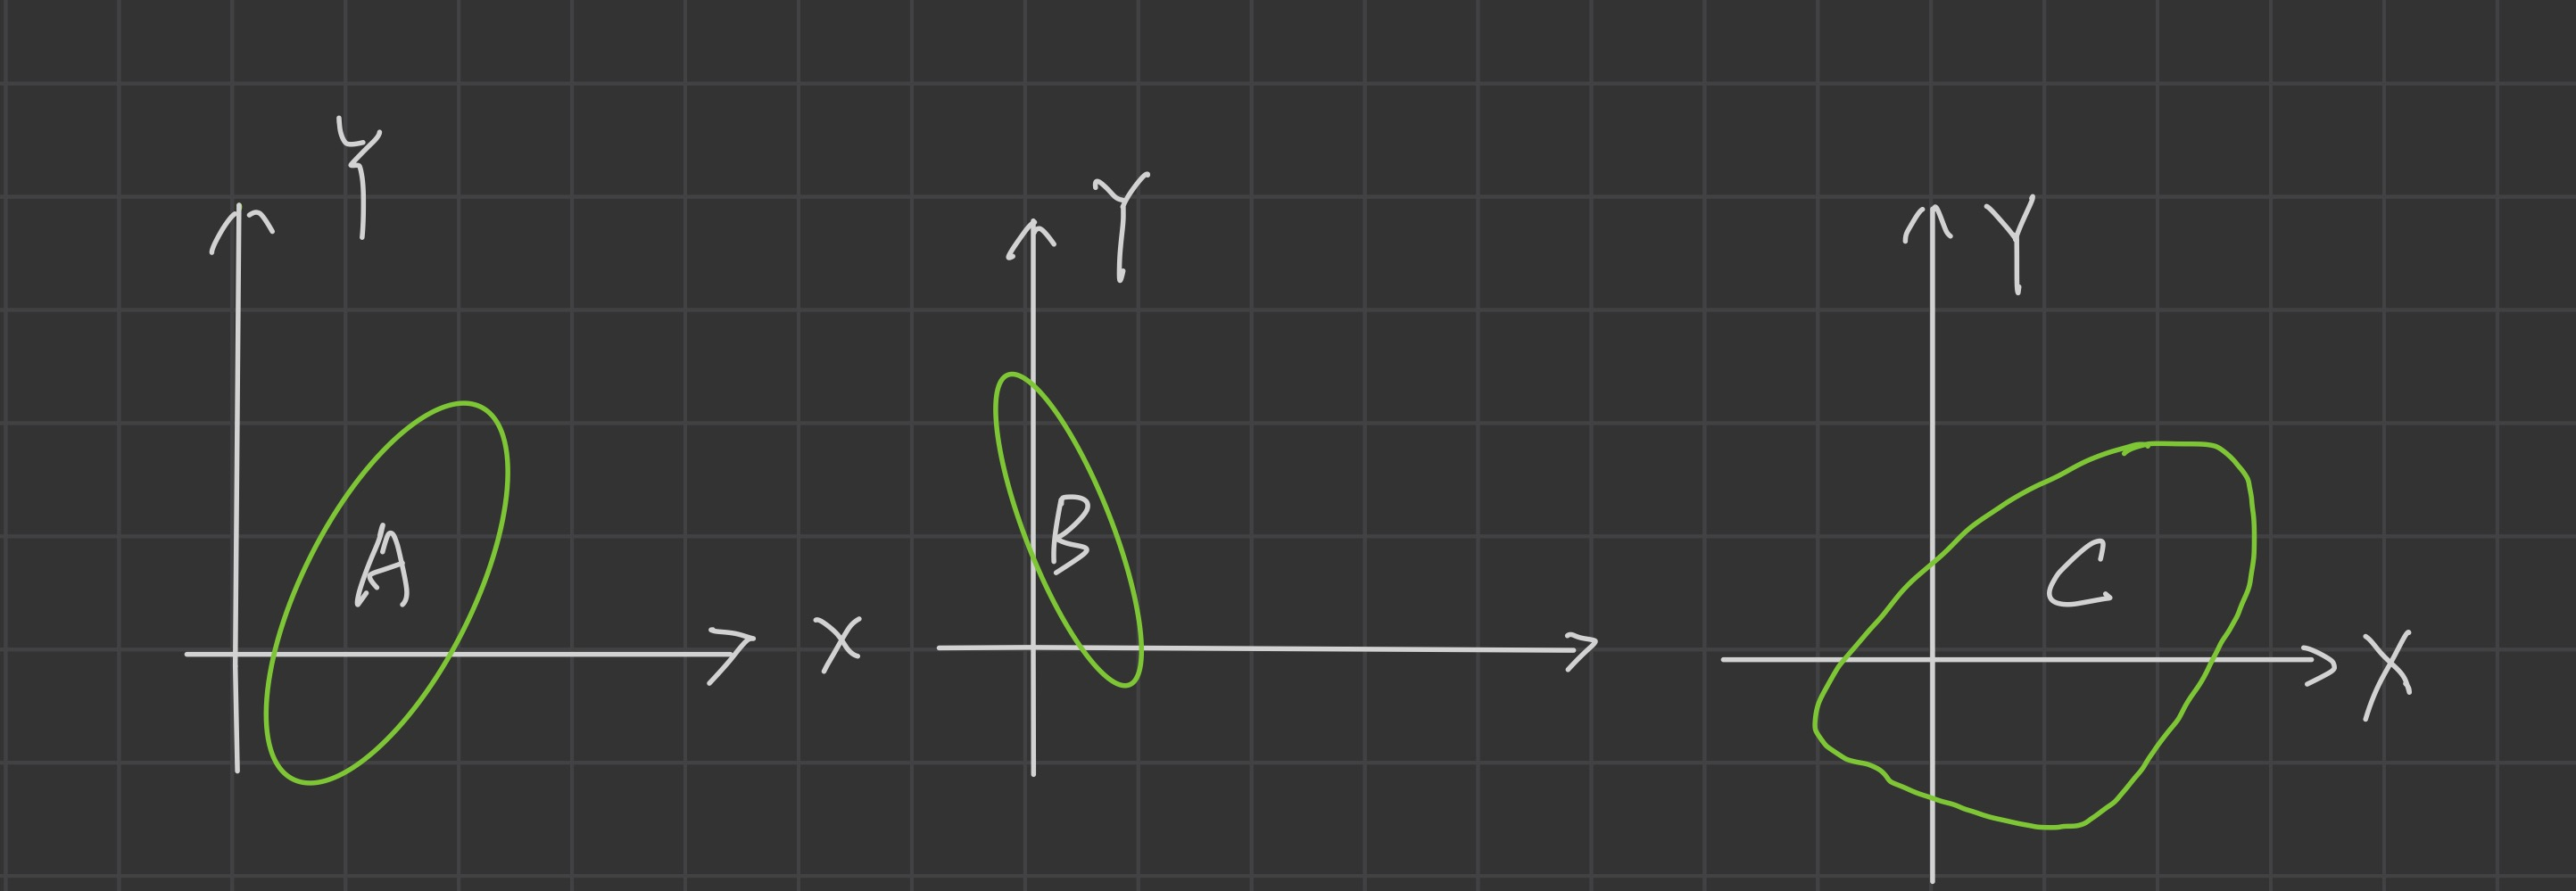
\includegraphics[width=10cm, height=4cm]{images/covariance.jpg}
\end{center}
\end{annotation}

\begin{proposition}
\rm \redt{最小二乘下的线性逼近} 设有两个随机变量$X,Y$. 给定两个实数$a,b$,若要使得$E\left\{\left[Y-(aX+b) \right]^2\right\}$达到最小,则得
$$
a  = \frac{\text{Cov}(X,Y)}{D(X)}
$$
和
$$
b = E(Y)-E(X)\frac{\text{Cov}(X,Y)}{D(X)}.
$$
其对应的最小值为
$$
E\left\{\left[Y-(aX+b) \right]^2\right\} = (1-\rho_{XY}^2)D(Y).
$$
\end{proposition}

\begin{proof}
我们设$E(X)=m_1,E(Y)=m_2,D(X)=\sigma_1^2,D(X)=\sigma_2^2$. 于是
$$
E\left\{\left[Y-(aX+b) \right]^2\right\} = E\left\{\left[(Y-m_2)-a(X-m_1)+ m_2 -am_1 - b \right]^2\right\}.
$$
记$c = m_2 -am_1 - b$,则
$$
E\left\{\left[(Y-m_2)-a(X-m_1)+ c \right]^2\right\} = \sigma_2^2 + a^2\sigma_1^2-2a\text{Cov}(X,Y) + c^2 .
$$
对上式分布求偏导并令它们等于0,可得$c=0$和$a = \frac{\text{Cov}(X,Y)}{D(X)}$,由此马上可到
$$
b = m_2-am_1 = E(Y)-E(X)\frac{\text{Cov}(X,Y)}{D(X)}.
$$
带入$b,c$即得
$$
E\left\{\left[Y-(aX+b) \right]^2\right\} = \sigma_2^2 + \frac{[\text{Cov}(X,Y)]^2}{\sigma_1^2}-2\frac{[\text{Cov}(X,Y)]^2}{\sigma_1^2} = \sigma_2^2(1-\rho_{XY}^2).
$$
\end{proof}

\begin{proposition}
\rm \redt{线性变换不影响相关系数} 若随机$X$和$Y$的相关系数为$\rho_{XY} \neq 0$,那么$Y$和$aX+b$的相关系数等于$\frac{a}{|a|}\rho_{XY}$,其中$a \neq 0$. 
\end{proposition}

\subsection{常用分布的数字特征}

\begin{proposition}
\rm 设$X$服从参数为$p$的\redt{两点分布},则$X$的期望为$E(X) = p$,方差为$p(1-p)$.
\end{proposition}

\begin{proof}
$X$期望为
$$
E(X) = 1\cdot p + 0 \cdot (1-p) = p.
$$
其方差为
$$
D(X) = (1-p)^2 \cdot p + (0-p)^2 (1-p) = (1-p)(p)(1-p+p) = p(1-p). 
$$
\end{proof}

\begin{proposition}
\rm 设\redt{$X \sim B(n,p)$},则$X$的期望为$np$,方差为$np(1-p)$.
\end{proposition}

\begin{proof}
设$q = 1-p$,$X$期望为
$$
E(X) = \sum\limits_{k=1}^n kC_n^kp^kq^{n-k} = \sum\limits_{k=1}^n k\cdot\frac{n!}{k!(n-k)!}p^kq^{n-k} = np \sum\limits_{k=1}^n C_{n-1}^{k-1}p^{k-1}q^{(n-1)-(k-1)} =np \sum\limits_{k'=0}^{n-1} C_{n-1}^{k'}p^{k'}q^{(n-1)-k'} = np. 
$$
其方差为
$$
D(X) = E(X^2) -E^2(X) = np\sum\limits_{k'=0}^{n-1} (k'+1) C_{n-1}^{k'}p^{k'}q^{(n-1)-k'} -n^2p^2= np(n-1)p + np - n^2p^2 = np(1-p).
$$
\end{proof}

\begin{proposition}
\rm 设\redt{$X \sim P(\lambda)$},则$X$的期望为$\lambda$,方差为$\lambda$.
\end{proposition}

\begin{proof}
$X$的期望为
$$
E(X) = \sum\limits_{k=0}^{\infty} k\cdot \frac{\lambda ^k}{k!}e^{-\lambda} =  \lambda \sum\limits_{k=1}^{\infty}  \frac{\lambda ^{k-1}}{(k-1)!}e^{-\lambda} = \lambda.
$$
其方差为
$$
\begin{array}{ll}
D(X) &= \sum\limits_{k=0}^{\infty} (k-\lambda)^2 \frac{\lambda ^k}{k!}e^{-\lambda} \\ 
&= \sum\limits_{k=0}^{\infty} (k^2 - 2k\lambda + \lambda^2) \frac{\lambda ^k}{k!}e^{-\lambda} \\ 
&= \sum\limits_{k=1}^{\infty} \lambda (k-1+1) \cdot \frac{\lambda ^{k-1}}{(k-1)!}e^{-\lambda}  - 2\lambda^2 +\lambda^2\\
&= \lambda^2 + \lambda - 2\lambda^2 + \lambda^2 = \lambda
\end{array}
$$
\end{proof}

\begin{proposition}
\rm 设$X$服从参数为$p$的\redt{几何分布},则$X$的期望为$\frac{1}{p}$,方差为$\frac{(1-p)}{p^2}$.
\end{proposition}

\begin{proof}
设$q= 1- p$,$X$的期望为
$$
E(X) = \sum\limits_{k=1}^\infty k \cdot q^{k-1}p = p(\sum\limits_{k=1}^\infty q^{k})' = p \left[\lim\limits_{n \to \infty}\frac{q(1-q^n)}{1-q} \right]' = p\left[\frac{q}{1-q}\right]' = p \cdot \frac{1}{(1-q)^2} = \frac{1}{p}. 
$$
其方差为
$$
\begin{array}{ll}
D(X) &= E(X^2)-E^2(X) \\
&= \left(\sum\limits_{k=1}^\infty k^2 \cdot q^{k-1}p \right) -\frac{1}{p^2} \\
&= p\left(\sum\limits_{k=1}^{\infty} kq^k\right)' - \frac{1}{p^2} \\
&= p\left[ q \left(\sum\limits_{k=1}^{\infty} q^k \right)'\right]' -\frac{1}{p^2}\\
&= p \cdot \frac{(1-q)(1+q)}{(1-q)^4} - \frac{1}{p^2} \\
&= \frac{1+q}{p^2} - \frac{1}{p^2} = \frac{q}{p^2}
\end{array}
$$
\end{proof}

\begin{proposition}
\rm 设$X$服从参数为$n,N,M$的\redt{超几何分布}($n \leq N-M$),则$X$的期望为$\frac{nM}{N}$,方差为$\frac{nM}{n} \frac{(N-M)}{N} \frac{N-n}{N-1}$. 
\end{proposition}

\begin{proof}
$X$的期望为
$$
\begin{array}{ll}
E(X) &= \sum\limits_{m=0}^{\min(M,n)} m \cdot \frac{C_M^mC_{N-M}^{n-m}}{C_N^n} \\
&= \sum\limits_{m=0}^{\min(M,n)} m \cdot \frac{M!}{m!(M-m)!} \cdot \frac{(N-M)!}{(n-m)![(N-M)-(n-m)]!} \cdot \frac{n!(N-n)!}{N!} \\
&= \sum\limits_{m=0}^{\min(M,n)} \frac{M(M-1)!}{(m-1)![(M-1)-(m-1)]} \cdot  \frac{[(N-1)-(M-1)]!}{[(n-1)-(m-1)]![(N-1)-(M-1)-((n-1)-(m-1))]!} \cdot \frac{n(n-1)![(N-1)-(n-1)]!}{N(N-1)!} \\
&= \frac{nM}{N} \sum\limits_{m'=0}^{\min(M-1,n-1)} \frac{C_{M-1}^{m'}C_{(N-1)-(M-1)}^{(n-1)-m'}}{C_{N-1}^{n-1}}\\
&= \frac{nM}{N} 
\end{array}
$$
其方差为
$$
D(X) = E(X^2) - E^2(X).
$$
%TODO
\end{proof}

\begin{proposition}
\rm 设$X$服从区间$[a,b]$上的\redt{均匀分布},则$X$期望为$\frac{a+b}{2}$,方差为$\frac{(b-a)^2}{12}$.
\end{proposition}

\begin{proof}
\rm $X$的期望为
$$
E(X) = \int_{a}^{b} x\cdot\frac{1}{b-a}dx = \left. \frac{x^2}{2(b-a)} \right\vert_{a}^{b} = \frac{a+b}{2}. 
$$
其方差为
$$
D(X) = \int_{a}^{b} \left(x-\frac{a+b}{2}\right)^2 \cdot\frac{1}{b-a}dx = \left. \left[ \frac{1}{b-a} \left( \frac{x^3}{3} - \frac{a+b}{2}x^2 +\frac{(a+b)^2}{4}x  \right)\right]\right\vert_{a}^{b} = \frac{(b-a)^2}{12}.
$$
\end{proof}

\begin{proposition}
\rm 设\redt{$X \sim E(\lambda)$},则$X$的期望为$\frac{1}{\lambda}$,方差为$\frac{1}{\lambda^2}$. 
\end{proposition}

\begin{proof}
$X$的期望为
$$
E(X) = \int_{0}^{+\infty} x\cdot \lambda e^{-\lambda x} dx = \frac{1}{\lambda}\int_{0}^{+\infty} t e^{-t} dx = \frac{1}{\lambda} \left[ \left. (-te^{-t}) \right\vert_{0}^{+\infty} + \int_{0}^{+\infty} e^{-t}dt \right] = \frac{1}{\lambda}.
$$
其方差为
$$
D(X) = E(X^2) - E^2(X) = \left[\int_{0}^{+\infty} x^2 \cdot \lambda e^{-\lambda x} dx \right] - \frac{1}{\lambda} = \left[ \frac{1}{\lambda^2} \int_{0}^{+\infty} \lambda^2 x^2 e^{-\lambda x}dx \right]-\frac{1}{\lambda^2},
$$
其中,令$t = \lambda x$
$$
\frac{1}{\lambda} \int_{0}^{+\infty} \lambda^2 x^2 e^{-\lambda x}dx = \frac{1}{\lambda^2} \int_{0}^{+\infty} t^2e^{-t}dt = \frac{1}{\lambda^2} \Gamma(3) =\frac{2}{\lambda^2}.
$$
故$D(X)=\frac{1}{\lambda^2}$
\end{proof}

\begin{corollary}
\rm 设$X \sim E(\lambda)$,则$E(X^n) = \frac{n!}{\lambda^n}$.
\end{corollary}

\begin{proposition}
\rm 设\redt{$X \sim N(\mu,\sigma^2)$},则$X$的期望为$\mu$,方差为$\sigma^2$,二阶原点矩为$\sigma^2+\mu^2$.
\end{proposition}

\begin{proof}
$X$的期望可以由\ref{expectation-of-symmetry}得知. 其方差为
$$
\begin{array}{llr}
D(X) &= \int_{-\infty}^{+\infty} (x-\mu)^2 \cdot \frac{1}{\sqrt{2\pi}\sigma} e^{-\frac{(x-\mu)^2}{2\sigma^2}}dx  \\
&= \int_{-\infty}^{+\infty} \sigma^2 t^2 \cdot \frac{1}{\sqrt{2\pi}\sigma} e^{-\frac{t^2}{2}} & \text{令}~t=\frac{x-\mu}{\sigma} \\
&=\sigma^2
\end{array}
$$
其二阶原点阶为
$$
E(X^2) = D(X)+E^2(X) =  \sigma^2 + \mu^2.
$$
\end{proof}



%regular_distribution_characterize.jpg
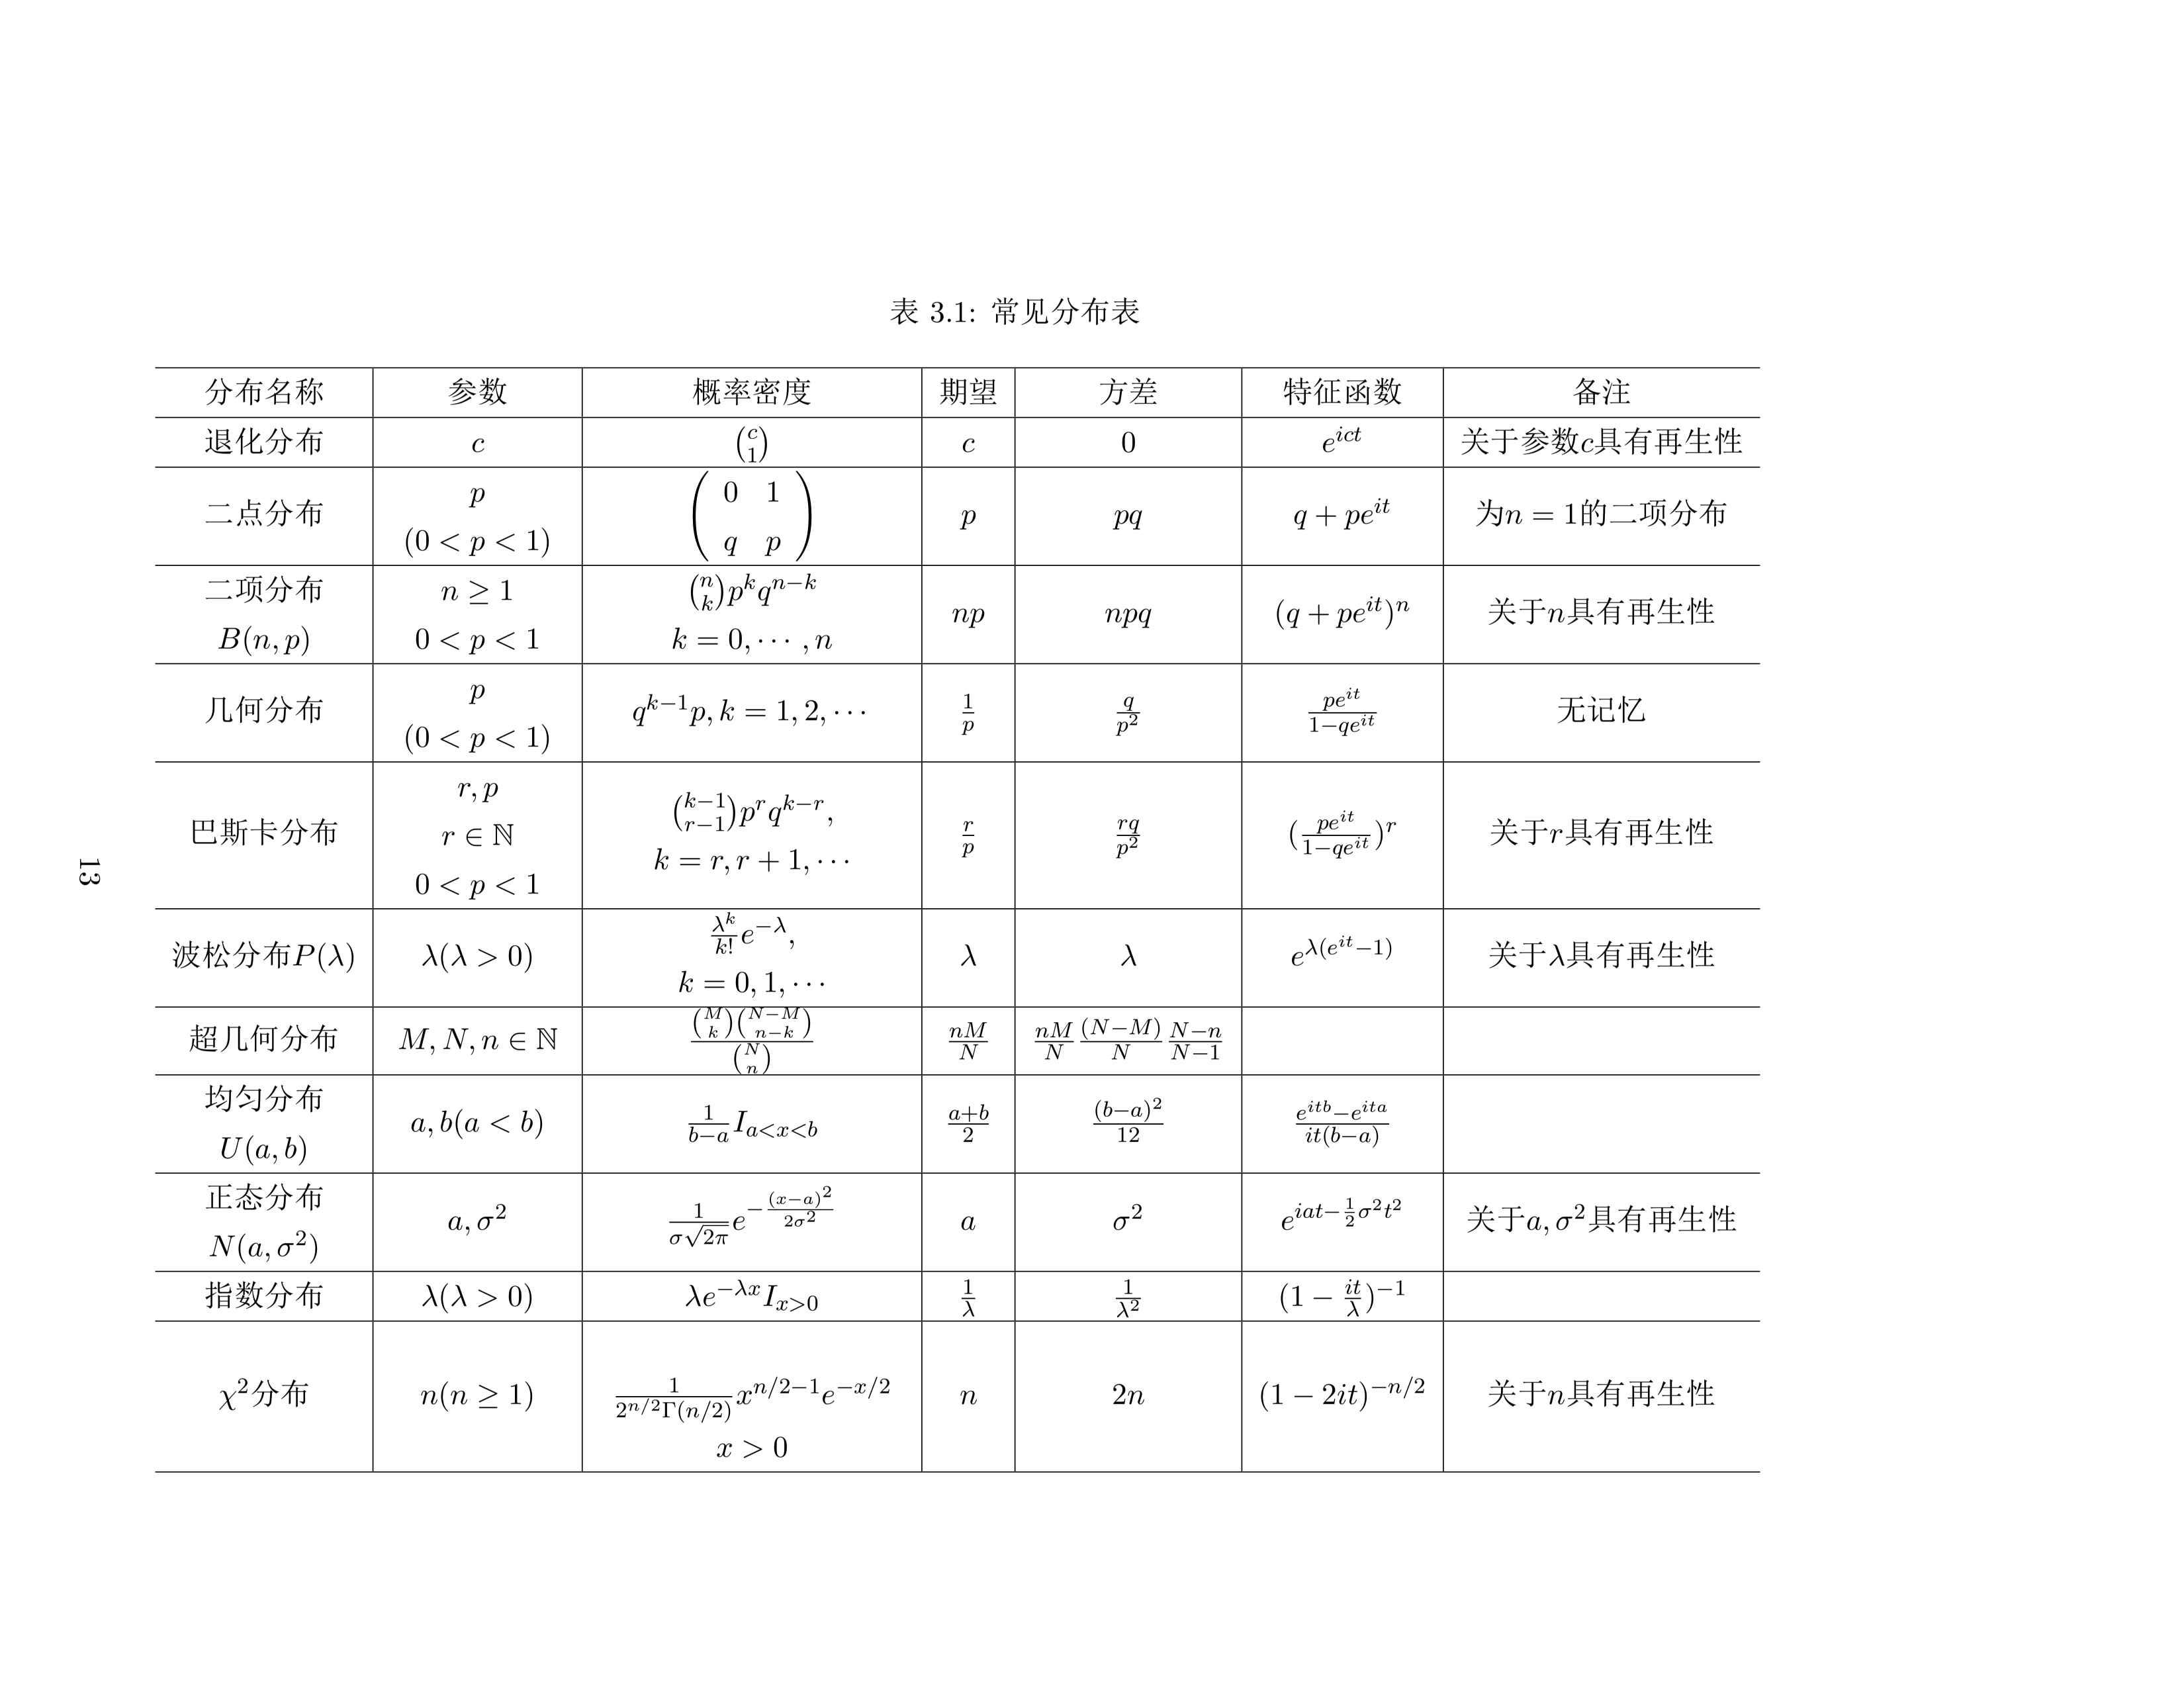
\includegraphics[scale=0.2]{images/regular_distribution_characterize.jpg}


\newpage
\section{大数定理和中心极限定理}

\begin{theorem}
\rm \redt{(切比雪夫不等式)} 设随机变量$X$具有数学期望$E(X)=\mu$,方差为$D(X) = \sigma^2$,则有
$$
P\{|X-\mu| \geq \varepsilon \} \leq \frac{\sigma^2}{\varepsilon^2}. 
$$
\end{theorem}

\begin{proof}
若$X$是连续性随机变量,其概率密度为$f(x)$,则
$$
P\{|X-\mu| \geq \varepsilon \} = \int_{|x-u| \geq \varepsilon} f(x)dx \leq \int_{|x-u| \geq \varepsilon} \frac{(x-\mu)^2}{\varepsilon^2}f(x)dx \leq \frac{1}{\varepsilon^2}\int_{-\infty}^{+\infty}(x-\mu)^2f(x)dx =\frac{\sigma^2}{\varepsilon^2}
$$
\end{proof}

\begin{annotation}
\rm 切比雪夫不等式用于在已知$E(X)$和$D(X)$的情况下估计概率$P\{|X-\mu|\geq \varepsilon\}$. 
\end{annotation}

\begin{theorem}
\rm \redt{(马尔科夫不等式)} 设$X$为非负随机变量,则对任意数$\varepsilon > 0$有
$$
P\{X \geq \varepsilon\} \leq \frac{E(X)}{\varepsilon}.
$$
\end{theorem}

\begin{proof}
若$X$是连续性随机变量,其概率密度为$f(x)$. 因$X$非负,所以有$y < 0,f(y)=0$,故
$$
E(X) = \int_{0}^{+\infty} xf(x)dx \geq  \int_{\varepsilon}^{+\infty} xf(x)dy.
$$
当$x \in [\varepsilon,+\infty]$,有$x \geq \varepsilon$. 于是有
$$
E(X) \geq \int_{\varepsilon}^{+\infty} xf(x)dx \geq \varepsilon \int_{\varepsilon}^{+\infty}f(x)dx = \varepsilon P\{X \geq \varepsilon\}.
$$
\end{proof}

\begin{theorem}
\rm \redt{(辛钦大数定理)} 设$X_1,X_2,\cdots,X_n,\cdots$是独立同分布的随机变量,即$E(X_i) = \mu,i=1,2,\cdots$. 则对任意数$\varepsilon > 0$有
$$
\lim\limits_{n \rightarrow \infty}P\{|\overline{X}_n -\mu| \geq \varepsilon\} = 0,
$$ 
其中$\overline{X}_n = \frac{\sum\limits_{i=1}^n X_i}{n}$. 
\end{theorem}

\begin{proof}
设$D(X_i) = \sigma^2, i =1,2,\cdots$. 由切比雪夫不等式有
$$
P\{|\overline{X}_n -\mu| \geq \varepsilon\} \leq \frac{D(\overline{X}_n)}{\varepsilon^2} = \frac{n\frac{\sigma^2}{n^2}}{\varepsilon^2} = \frac{\sigma^2}{n\varepsilon^2}. 
$$
因此
$$
\lim\limits_{n \rightarrow \infty} P\{|\overline{X}_n -\mu| \geq \varepsilon\} = \lim\limits_{n \rightarrow \infty} \frac{\sigma^2}{n\varepsilon^2} = 0.
$$
\end{proof}

\begin{proposition}
\rm \redt{伯努利大数定理} 若随机变量$S_n \sim B(n,p)(n=1,2,\cdots)$,则对于任意$\varepsilon > 0$,有
$$
\lim\limits_{n \rightarrow \infty}P\left\{\left|\frac{S_n}{n} -p\right| \geq \varepsilon\right\} = 0.
$$
其中$S_n = X_1+X_2+\cdots+X_n$. \bluet{频率趋于概率}. 
\end{proposition}

\begin{proof}
\rm 上述命题描述的是随机变量$X_1,X_2,\cdots,X_n$是相互独立且条件相同的试验,设一次试验下$A$发生的概率为$p$,那么可以理解为
$$
X_i = \left\{  \begin{array}{ll}
1 & \text{第$i$试验时$A$发生}\\
0 & \text{第$i$试验时$A$不发生}\\
\end{array}  \right.
$$ 
所以实际上$X_1,X_2,\cdots,X_n$就是一个$n$重伯努利试验,记为$S_n \sim B(n,p)$. 对任意一次试验的期望为$E(X_i) = p$,由大数定理最终有
$$
\lim\limits_{n \rightarrow \infty}P\left\{\left|\frac{S_n}{n} -p\right| \geq \varepsilon\right\} = 0.
$$ 
\end{proof}

\begin{theorem}
\rm \redt{更一般的切比雪夫大数定理} 设$X_1,X_2,\cdots,X_n,\cdots$为相互独立的随机变量,它们的期望$E(X_i)$和方差$D(X_i)$都存在,而且方差上有界,即$D(X_i) \leq L, i = 1,2,\cdots$. 则对任意的$\varepsilon > 0$,都有
$$
\lim\limits_{n \to \infty} P\left\{ \left| \frac{1}{n} \sum\limits_{i=1}^n X_i - \frac{1}{n} \sum\limits_{i=1}^n E(X_i) \right| \geq \varepsilon \right\} = 0. 
$$
\end{theorem}

\begin{definition}
\rm 设$\xi_n, n = 1,2,\cdots$为随机变量序列,$\xi$为随机变量(可以为常数),若$\forall \varepsilon > 0$,有
$$
\lim\limits_{n \to \infty} P\{ |\xi_n -\xi| > \varepsilon \} = 0
$$
成立,则称$\xi_n$\redt{依概率收敛}到$\xi$,记做
$$
\xi_n \xrightarrow{\text{Pr}} \xi.
$$
\end{definition}


\begin{theorem}
\rm \redt{中心极限定理(列维-林德伯格定理)} 设$X_1,X_2,\cdots,X_n,\cdots$为独立同分布的随机变量,$E(X_i)=\mu,D(X_i)=\sigma^2,i=1,2,\cdots$. 则对任意实数$x$,有
$$
\lim\limits_{n \rightarrow \infty}P\left\{\frac{1}{\sqrt{n}\sigma}\left(\sum\limits_{i=0}^nX_i - n\mu \right) \leq x\right\} = \Phi(x)
$$
这里$\Phi(x)$是标准正态分布$N(0,1)$的分布函数. 
\end{theorem}



\begin{annotation}
\rm 注意$\frac{1}{\sqrt{n}\sigma}(\sum\limits_{i=0}^nX_i - n\mu)$的期望为$0$方差为$1$,这个操作称为$X_1 + X_2 +\cdots + X_n$的标准化,即与$N(0,1)$的期望和方差符号. 
\end{annotation}

\begin{theorem}
\rm \redt{中心极限定理的一个特例(拉普拉斯中心极限定理)} 设随机变量$S_n \sim B(n,p)(n=1,2,\cdots)$,则对于任意的实数$x$,有
$$
\lim\limits_{n \rightarrow \infty}P\left\{\frac{1}{\sqrt{np(1-p)}}(S_n - np) \leq x\right\} = \Phi(x),
$$
其中$S_n = X_1+X_2+\cdots + X_n$. \bluet{在$n$充分大的时候,将$S_n$标准化之后其分布近似等于标准正态分布}. 
\end{theorem}


\newpage
\section{数理统计的基本概念}

\subsection{总体、样本、统计量和样本数字特征}

\begin{definition}
\rm 对推断统计而言,主要有如下两大类:
\begin{enumerate}
	\item \redt{参数估计} 在概率模型(分布)假定下,根据数据用一些方法对分布的位置参数进行估计. 
	\item \redt{假设检验} 对某种假设做出推断,即根据数据,用一些方法对分布或者分布中的未知数参数进行检验. 
\end{enumerate}
\end{definition}

\begin{definition}
\rm 数理统计中所研究对象的某项数量指标的全体称为\redt{总体},而把总体中的每个成员称为\redt{个体}.
\end{definition}

\begin{definition}
\rm 若用$X$表示所研究对象的某一指标随机变量,则总体即为$X$(的分布). 从总体中抽取的$n$个个体$X_1,\cdots,X_n$组成一个\redt{样本},$n$称为这个样本的\redt{样本容量},而样本$X_1,\cdots,X_n$的值$x_1,\cdots,x_n$称为样本的\redt{观察值}. 由于$X_1,X_2,\cdots,X_n$是从总体$X$随机抽取出来的可能结果,可以看成$n$个随机变量. 当$X_1,\cdots,X_n$独立同分布时,称为$X_1,\cdots,X_n$为\redt{简单样本}(后面若无特殊说明,所说的样本都是指简单样本).
\end{definition}

\begin{proposition}
\rm 若总体$X$的分布为$F(x)$,则样本$(X_1,\cdots,X_n)$的联合分布为
$$
F(x_1,\cdots,x_n) = \prod\limits_{i=1}^n F(x_i).
$$
若$X$是离散型随机变量,那么$(X_1,\cdots,X_n)$的联合概率分布为
$$
P\{X_1 = x_1 ,\cdots , X_n = x_n\} = \prod\limits_{i=1}^n P\{X=x_i\}.
$$
若$X$是连续随机变量,那么其$(X_1,\cdots,X_n)$的联合概率密度为
$$
f(x_1,\cdots,x_n) = \prod\limits_{i=1}^n f(x_i).
$$
\end{proposition}

\begin{definition}
\rm 关于样本$X_1,\cdots,X_n$的不含未知参数的函数$T=T(X_1,\cdots,X_n)$称为\redt{统计量}. \bluet{也就是只依赖样本的量称为统计量}. 统计量是随机函数,其分布叫做抽样分布. 
\end{definition}

\begin{definition}
\rm 常见的统计量
\begin{enumerate}
	\item 样本均值 $\bar{X} = \frac{1}{n}\sum\limits_{i=1}^n X_i$,反映了总体总结的信息. 
	%https://www.zhihu.com/question/20099757 为什么样本方差(sample variance)的分母是 n-1?
	\item 样本方差 $S^2 = \frac{1}{n-1}\sum\limits_{i=1}^n(X_i-\bar{X})^2$,反映了总体方差的信息.
	\item 样本$k$阶原点矩$A_k = \frac{1}{n}\sum\limits_{i=1}^n X_i^k$,反映了总体$k$阶原点矩的信息.
	\item 样本$k$阶中心矩$B_k = \frac{1}{n}\sum\limits_{i=1}^n (X_i-\bar{X})^k$,反映了总体$k$阶中心矩的信息. 特别地$B_2 = \frac{n-1}{n}S^2$.
\end{enumerate}
\end{definition}

\begin{proposition}
\rm 样本均值$\overline{X}$的期望和方差为 
$$
E(\overline{X}) = E(X), D(\overline{X})=\frac{D(X)}{n}.
$$
\end{proposition}

\begin{proposition}\label{sample-variance-expand}
\rm 
$$
\sum\limits_{i = 1}^n (X_i - \overline{X})^2 = \sum\limits_{i = 1}^n X_i^2 -  n\overline{X}^2 
$$
\bluet{样本方差的一个展开式,再对其求期望你会发现很简单}. 
\end{proposition}

\begin{proof}
$$
\begin{array}{ll}
\sum\limits_{i = 1}^n (X_i - \overline{X})^2 &= \sum\limits_{i = 1}^n (X_i^2 - 2X_i\overline{X} + \overline{X}^2)  \\
&=  \sum\limits_{i = 1}^n X_i^2 - 2\overline{X} \sum\limits_{i = 1}^n X_i + n\overline{X}^2 \\
&= \sum\limits_{i = 1}^n X_i^2  - n\overline{X}^2\\
\end{array}
$$
\end{proof}

\begin{proposition}
\rm 
$$
E\left[ \sum\limits_{i = 1}^n  (X_i - \overline{X})^2 \right] = (n-1)D(X).
$$
\end{proposition}

\begin{proof}
\rm 直接用\ref{sample-variance-expand}的结论可以求,即
$$
E(\sum\limits_{i = 1}^n X_i^2  - n\overline{X}^2) = n\left[E^2(X) + D(X)\right]- n\left[\frac{D(X)}{n} + E^2(X)\right] = (n-1)D(X). 
$$
\end{proof}

\begin{proposition}\label{sample-mean-distribution}
\rm 设$X_1,X_2,\cdots,X_n$相互独立,且服从$N(\mu,\sigma^2)$,则
$$
\overline{X} \sim N(\mu,\frac{\sigma^2}{n}).
$$
\end{proposition}

\begin{definition}
\rm 将样本$X_1,\cdots,X_n$的观测值$x_1,\cdots,x_n$按大小排序,得到$x_{(1)} \leq \cdots x_{(n)}$,则称
$$
F_n(x) = \left\{
\begin{array}{ll}
0, & x <x_{(1)} \\
\frac{\lfloor x \rfloor}{n}, &  x_{(1)}\leq x \leq x_{(n)}\\
1, &x > x_{(n)}
\end{array} \right.
$$
为\redt{经验分布函数}.
\end{definition}

\subsection{统计三大分布}

\begin{definition}
\rm 设$X_1,\cdots,X_n$为相互独立且具有共同分布$N(0,1)$的随机变量,则称$X=\sum\limits_{i=1}^n X_i^2$的分布服从\redt{自由度为$n$的$\chi ^2$分布}(卡方分布),记为$X \sim \chi_n^2$.
\end{definition}

\begin{definition}
\rm 对于给定正数$\alpha, 0 <\alpha <1$,满足条件
$$
P\{\chi^2 > \chi_\alpha^2(n)\} = \int_{\chi_\alpha^2(n)}^{+\infty} = \alpha
$$
的点$\chi_\alpha^2(n)$称为$\chi^2(n)$分布上的\redt{$\alpha$分位点}. 
\end{definition}

\begin{lemma}\label{for-chi-proof}
\rm 设$X \sim N(0,1)$,则
$$
X^2 \sim \Gamma(\frac{1}{2},\frac{1}{2}). 
$$
\end{lemma}

\begin{proof}
见\ref{normal-distribution-square}. 
\end{proof}

\begin{proposition}
\rm $\chi_n^2$分布的概率密度为
$$
f(x) =  \left\{
\begin{array}{ll}
\frac{1}{2^\frac{n}{2}\Gamma(\frac{n}{2})} x^{\frac{n}{2}-1}e^{\frac{-x}{2}}, & x > 0 \\
0, & \text{other}
\end{array} \right. 
$$
\end{proposition}

\begin{proof}
由\ref{for-chi-proof}配合$\Gamma$分布的可加性\ref{gamma-distribution-additivity},则有$\chi^2 \sim \Gamma(\frac{n}{2},\frac{1}{2})$. 
\end{proof}

\begin{proposition}
\rm \redt{$\chi^2$分布的可加性} 设$\chi_1^2 \sim \chi^2(n_1),\chi_2^2 \sim \chi^2(n_2)$,且$\chi_1^2$和$\chi_2^2$相互独立,则
$$
\chi_1^2 + \chi_2^2 = \chi^2(n_1 + n_2). 
$$
\end{proposition}

\begin{proposition}
\rm \redt{$\chi^2$的数学期望和方差} 设$\chi^2 \sim \chi^2(n)$,则
$$
E(\chi^2) = n, D(\chi^2) = 2n
$$
\end{proposition}

\begin{proof}
先计算$X_i^2$的期望和方差
$$
\begin{array}{ll}
E(X_i^2) = E^2(X_i) + D(X_i) = 1 \\
D(X_i^2) = E(X_i^4) - E^2(X_i^2) = 3-1 = 2
\end{array}
$$
因此
$$
\begin{array}{ll}
E(\chi^2) = E(\sum\limits_{i=1}^n X_i^2) =\sum\limits_{i=1}^n E(X_i^2) = n \\
D(\chi^2) = D(\sum\limits_{i=1}^n X_i^2) =\sum\limits_{i=1}^n D(X_i^2) = 2n 
\end{array}
$$
\end{proof}


\begin{definition}
\rm 设随机变量$X$和$Y$相互独立,且$X \sim N(0,1), Y \sim \chi^2(n)$,则称随机变量
$$
T = \frac{X}{\sqrt{\frac{Y}{n}}}
$$
服从\redt{自由度为$n$的$t$分布},记做$T\sim t(n)$.
\end{definition}

\begin{proposition}
\rm $t(n)$分布的概率密度为
$$
h(t) =\frac{\Gamma(\frac{n+1}{2})}{\Gamma(\frac{n}{2})\cdot \sqrt{n\pi}}\left(1+\frac{t^2}{n}\right)^{-\frac{n+1}{2}}.
$$
\end{proposition}

\begin{proposition}
\rm $t$分布的概率密度$h(t)$是偶函数,即
$$
h(t)=h(-t).
$$
\end{proposition}

\begin{proposition}
\rm \redt{$t$分布在$n$很大时接近标准正态分布}
$$
\lim\limits_{n \to \infty} h(t) = \Phi(t),
$$
其中$\Phi(t)$是标准正态分布的概率密度. 
\end{proposition}

\begin{definition}
\rm 设随机变量$X$和$Y$相互独立,且$X \sim \chi^2(n_1), Y \sim \chi^2(n_2)$,则称随机变量
$$
F = \frac{\frac{X}{n_1}}{\frac{Y}{n_2}}
$$
服从\redt{自由度为$(n_1,n_2)$的$F$分布},记做$F \sim F(n_1,n_2)$,其中$n_1$和$n_2$称为第一自由度和第二自由度. 
\end{definition}

\begin{proposition}
\rm $F(m,n)$分布的概率密度为
$$
f_{m,n} = m^{\frac{m}{2}} n^{\frac{n}{2}} \frac{\Gamma(\frac{m+n}{2})}{\Gamma(\frac{m}{2})\Gamma(\frac{m}{2})}x^{\frac{m}{2}-1}(mx+n)^{-\frac{m+n}{2}}, ~ x> 0.
$$
\end{proposition}

\begin{proposition}
\rm 若$X \sim F(n_1,n_2)$,则$X^{-1} \sim F(n_2,n_1)$. 
\end{proposition}

\begin{proposition}
\rm \redt{$t$分布和$F$分布的联系} 设随机变量$X \sim t(n)$,则
$$
X^2 \sim F(1,n). 
$$
\end{proposition}

\subsection{三大分布的重要性质}

\begin{proposition}\label{sample-means-normalization}
\rm \redt{标准化} 设$X_1,X_2,\cdots,X_n$相互独立,且都服从$N(\mu,\sigma^2)$,则有
$$
\frac{\overline{X} - E(X_i)}{\sqrt{\frac{D(X_i)}{n}}} \sim N(0,1).
$$
\end{proposition}

\begin{proof}
\rm 由\ref{sample-mean-distribution}可知.
\end{proof}

\begin{proposition}\label{sample-variance-replace-variance}
\rm \redt{未知总体分布方差的情况下对期望估计的重要手段} 设$X_1,X_2,\cdots,X_n$相互独立,且都服从$N(\mu,\sigma^2)$,则有
$$
\frac{\overline{X} - E(X_i)}{\sqrt{\frac{S^2}{n}}} \sim t(n-1). 
$$
\end{proposition}

\begin{proof}
由\ref{sample-means-normalization}和\ref{sample-variance-and-variance}可知
$$
\frac{\overline{X}-E(X_i)}{\sqrt{\frac{\sigma^2}{n}}} \sim N(0,1),\frac{(n-1)S^2}{\sigma^2} \sim \chi^2(n-1).
$$
再由$t$分布的定义可知
$$
\left. \frac{\overline{X}-E(X_i)}{\sqrt{\frac{\sigma^2}{n}}} \right/ \sqrt{\frac{(n-1)S^2}{(n-1)\sigma^2}} \sim t(n-1).
$$
\end{proof}

\begin{proposition}
\rm 设$X_1,X_2,\cdots,X_n$相互独立,且都服从$N(\mu,\sigma^2)$,则$\overline{X}$和$S^2$相互独立. \bluet{这个结论是服务于\ref{sample-variance-replace-variance}}
\end{proposition}

\begin{proposition}\label{sample-variance-and-variance}
\rm \redt{对方差的估计的重要手段} 设$X_1,X_2,\cdots,X_n$相互独立,且都服从$N(\mu,\sigma^2)$,则有
$$
\frac{(n-1)S^2}{\sigma^2} \sim \chi^2(n-1). 
$$
\end{proposition}

\begin{proof}
\rm 其中
$$
(n-1)S^2 = \sum\limits_{i=1}^n (X_i-\overline{X})^2 = \sum\limits_{i=2}^n \xi_i^2 
$$
其中$\xi_i \sim N(0,\sigma^2)$. 这是一个比较有趣的结论,因此
$$
\frac{\xi_i^2}{\sigma^2} = \left(\frac{\xi_i}{\sigma}\right)^2,
$$
其中$\frac{\xi_i}{\sigma} \sim N(0,1)$. 
\end{proof}

\begin{proposition}
\rm \redt{对两个总体的方差之比估计的重要手段} 设$X_1,X_2,\cdots,X_{n_1}$与$Y_1,Y_2,\cdots,Y_{n_2}$分别来自正态总体分布$N(\mu_1,\sigma_1^2)$及$N(\mu_2,\sigma_2^2)$,且这两个样本相互独立. 则有
$$
\frac{S_1^2/S_2^2}{\sigma_1^2 / \sigma_2^2} \sim F(n_1 -1,n_2 -1). 
$$
\end{proposition}

\begin{proof}
由\ref{sample-variance-and-variance}和$F$分布定义可知
$$
\left. \frac{(n_1-1)S^2}{(n_1-1)\sigma_1^2} \right / \frac{(n_2-1)S^2}{(n_2-1)\sigma_2^2} \sim F(n_1-1,n_2-1).
$$
\end{proof}

\begin{proposition}\label{two-sample-mean-difference}
\rm 设$X_1,X_2,\cdots,X_{n_1}$与$Y_1,Y_2,\cdots,Y_{n_2}$分别来自正态总体分布$N(\mu_1,\sigma_1^2)$及$N(\mu_2,\sigma_2^2)$,且这两个样本相互独立. 则有
$$
\overline{X} - \overline{Y} \sim N(\mu_1 -\mu_2, \frac{\sigma_1^2}{n_1} + \frac{\sigma_2^2}{n_2}).
$$
上式经过标准化之后则有
$$
\frac{(\overline{X} - \overline{Y})-(\mu_1-\mu_2)}{\sqrt{\frac{\sigma_1^2}{n} + \frac{\sigma_2^2}{n}}} \sim N(0,1).
$$
\end{proposition}

\begin{proposition}
\rm \redt{对两个总体的期望之差估计的重要手段} 设$X_1,X_2,\cdots,X_{n_1}$与$Y_1,Y_2,\cdots,Y_{n_2}$分别来自正态总体分布$N(\mu_1,\sigma_1^2)$及$N(\mu_2,\sigma_2^2)$,且这两个样本相互独立,且有$\sigma_1^2 = \sigma_2^2$,则有
$$
\frac{(\overline{X} - \overline{Y})-(\mu_1-\mu_2)}{S_\omega\sqrt{\frac{1}{n_1} + \frac{1}{n_2}}}\sim t(n_1+n_2-2),
$$
其中$S_\omega^2 = \frac{(n_1-1)S_1^2+(n_2-1)S_2^2}{n_1+n_2-2}$. 
\end{proposition}

\begin{proof}
设$\sigma_1^2 = \sigma_2^2 = \sigma^2$,由\ref{two-sample-mean-difference}有
$$
U = \frac{(\overline{X} - \overline{Y})-(\mu_1-\mu_2)}{\sigma\sqrt{\frac{1}{n_1} + \frac{1}{n_2}}} \sim N(0,1).
$$
由\ref{sample-variance-and-variance}和$\chi^2$分布的可加性有
$$
V = \frac{(n_1-1)S_1^2}{\sigma^2} + \frac{(n_2-1)S_2^2}{\sigma^2} = \frac{(n_1-1)S_1^2+(n_2-1)S_2^2}{\sigma^2} \sim \chi^2(n_1+n_2-2).   
$$
再结合$t$分布的定义,最终有
$$
\frac{U}{\sqrt{\frac{V}{n_1+n_2-2}}} = \frac{(\overline{X} - \overline{Y})-(\mu_1-\mu_2)}{S_\omega\sqrt{\frac{1}{n_1} + \frac{1}{n_2}}} \sim t(n_1+n_2-2). 
$$
\end{proof}

\newpage
\section{参数估计}

\subsection{点估计}

\begin{definition}
\rm 设有一个总体$X$,以$f(x,\theta_1,\cdots,\theta_k)$记其概率密度函数(若总体分布为连续型)或者概率函数(若总体分为为离散型),其中$\theta_1,\cdots,\theta_k$表示总体分布包含的$k$个未知参数,用样本$X_1,\cdots,X_n$构造的统计量$\widehat{\theta}_i(X_1,\cdots,X_n)$来估计未知参数$\theta_i$称为\redt{点估计},统计量$\widehat{\theta}_i(X_1,\cdots,X_n)$来估计未知参数称为\redt{估计量}.
\end{definition}

\begin{annotation}
\rm 前面的样本期望,方差和原点矩等等统计量都是点估计. 
\end{annotation}

\subsection{矩估计}

\begin{definition}
\rm 设总体$X$的分布有未知参数$\theta_1,\cdots,\theta_k$,抽取样本$X_1,\cdots,X_n$的观测值为$x_1,\cdots,x_2$. 设其有$l$阶原点矩$a_l$存在,设样本的$l$阶原点矩为$A_l = \frac{1}{n}\sum\limits_{i = 1}^n x_i ^l$. 于是
$$
a_l = a_l(\theta_1,\cdots,\theta_k) \approx A_l,
$$
取$l=1,2,\cdots,k$,就得到一个方程组,解此方程组,得其根为
$$
\widehat{\theta_i} = \widehat{\theta_i}(X_1,\cdots,X_n),i=1,2,\cdots,k.
$$
以$\widehat{\theta_i}$作为$\theta_i$的一个估计,这样的估计量叫做\redt{矩估计}. \bluet{即仅使用样本矩的点估计来构造方程}. 
\end{definition}

\begin{example}
\rm 设$X \sim N(u,\sigma^2)$,抽取样本$X_1,X_2,\cdots,X_n$的观测值为$x_1,x_2,\cdots,x_n$. 那么$X$的一阶原点矩和二阶原点矩为
$$
\begin{array}{ll}
E(X) = \mu \\
E(X^2) = \sigma^2 + \mu^2
\end{array}
$$
则构造的矩估计的方程组为
$$
\begin{array}{ll}
\mu = \frac{1}{n}\sum\limits_{i = 1}^n x_i \\
\sigma^2 + \mu^2 = \frac{1}{n}\sum\limits_{i = 1}^n x_i^2 
\end{array}
$$
解得
$$
\begin{array}{ll}
\widehat{\mu} = \frac{1}{n}\sum\limits_{i = 1}^n x_i =\overline{x} \\
\widehat{\sigma}^2 = \frac{1}{n}\left(\sum\limits_{i = 1}^n x_i^2 - n\overline{x}^2 \right) = \frac{1}{n}  \sum\limits_{i = 1}^n (x_i - \overline{x})^2
\end{array}
$$
\end{example}

\subsection{最大似然估计}

\begin{definition}
\rm 设总体$X$有分布$f(x;\theta_1,\cdots,\theta_k)$(即概率密度或者概率分布),给定样本$X_1,\cdots,X_n$的观察值$x_1,x_2,\cdots,x_n$,令
$$
L_n(x_1,x_2,\cdots,x_n;\theta_1,\cdots,\theta_k) = f(x_1;\theta_1,\cdots,\theta_k)f(x_2;\theta_1,\cdots,\theta_k)\cdots f(x_3;\theta_1,\cdots,\theta_k),
$$
称其为\redt{似然函数}(likelihood). 这函数对不同的$(\theta_1,\cdots,\theta_k)$的取值,反映了在观察结果$(x_1,\cdots,x_n)$已知的条件下,$(\theta_1,\cdots,\theta_k)$的各种值的似然程度. 应用似然程度最大$\max{L_n}$的那个$(\widehat{\theta_1},\cdots,\widehat{\theta_k})$作为$(\theta_1,\cdots,\theta_k)$的估计值. 这个估计$(\widehat{\theta_1},\cdots,\widehat{\theta_k})$就叫做$(\theta_1,\cdots,\theta_k)$的最大似然估计. 
\end{definition}

\begin{annotation}
\rm \bluet{多元函数求极值的场景}.
\end{annotation}

\begin{example}
\rm 设$X_1,\cdots,X_n$是从正态总体$N(\mu,\sigma^2)$中抽出的样本,其观测值为$x_1,\cdots,x_n$,则似然函数为
$$
L = \left(\frac{1}{\sqrt{2\pi}\sigma}\right)^ne^{\frac{-1}{2\sigma^2}\sum\limits_{i =1}^n (x_i-\mu)^2}.
$$
等式两边取对数有
$$
\ln L =-\frac{n}{2}\ln(2\pi)-\frac{n}{2}\ln(\sigma^2) - \frac{1}{2\sigma^2}\sum\limits_{i =1}^n (x_i-\mu)^2.
$$
于是
$$
\left\{
\begin{array}{ll}
\frac{\partial L}{\partial \mu} = \frac{1}{\sigma^2}\sum\limits_{i =1}^n (x_i-\mu) = 0 \\
\frac{\partial L}{\partial \sigma^2} = - \frac{n}{2\sigma^2} +\frac{1}{2(\sigma^2)^2} \sum\limits_{i =1}^n (x_i-\mu)^2 = 0
\end{array}\right.
$$
显然有$\widehat{\mu} = \bar{X} = \frac{\sum\limits_{i =1}^n x_i}{n}$,$\widehat{\sigma^2} = \frac{1}{n}\sum\limits_{i =1}^n (x_i-\bar{x})^2$. 我们还需要判定其是不是最大值,其二阶导分别为
$$
\left\{
\begin{array}{ll}
\frac{\partial^2L}{\partial \mu\partial \mu} = -\frac{n}{\sigma^2} \\
\frac{\partial^2L}{\partial \mu \partial \sigma^2} =  -\frac{1}{(\sigma^2)^2}\sum\limits_{i =1}^n (x_i-\mu) \\
\frac{\partial^2L}{\partial \sigma^2 \partial \mu} = -\frac{1}{(\sigma^2)^2}\sum\limits_{i =1}^n (x_i-\mu) \\
\frac{\partial^2L}{\partial \sigma^2 \partial \sigma^2} =  \frac{n}{2(\sigma^2)^2} - \frac{1}{(\sigma^2)^3}\sum\limits_{i =1}^n (x_i-\mu)^2
\end{array}\right.
$$
故$L$有二阶连续偏导,根据极值判定法则
$$
L_{\mu\mu}''(\widehat{\mu},\widehat{\sigma^2})\cdot L_{\sigma^2\sigma^2}''(\widehat{\mu},\widehat{\sigma^2}) - \left[L_{\mu\sigma^2}''(\widehat{\mu},\widehat{\sigma^2})\right]^2 = \frac{-n}{\widehat{\sigma^2}}\cdot\frac{-n}{2(\widehat{\sigma^2})^2} > 0.
$$
确实在$(\widehat{\mu},\widehat{\sigma^2})$取得最大值.
\end{example}

\begin{example}
\rm 设$X_1,\cdots,X_n$是从指数分布$E(\lambda)$中抽出的样本,则似然函数为
$$
L(x_1,\cdots,x_n;\lambda) = \lambda^n e^{-\lambda\sum\limits_{i=1}^{n} x_i}. 
$$
等式两边取对数则有
$$
\ln L = n\ln\lambda - \left(\lambda\sum\limits_{i=1}^{n} x_i\right). 
$$
于是
$$
\frac{dL}{d\lambda} = \frac{n}{\lambda} - \sum\limits_{i=1}^{n} x_i. 
$$
当$\lambda = \frac{n}{\sum\limits_{i=1}^{n} x_i}$时,$L$有最大值. 
\end{example}

\begin{example}
\rm 设总体$X \sim U[-\theta,\theta]$($\theta >0$),$X_1,X_2,\cdots,X_n$是来自总体$X$的简单随机样本. 则似然函数为
$$
L(\theta) = \prod_{i=1}^{n} = \left\{ \begin{array}{ll}
\frac{1}{(2\theta)^n} & -\theta \leq x_1,x_2,\cdots,x_n \leq \theta \\
0 & \text{其他}
\end{array} \right.
$$
显然,当$\theta$越小$L(\theta)$就越大,但是需要注意的是$[-\theta,\theta]$必须把样本中所有的点盖住. 因此我们应该选取$[-\theta,\theta]$盖住样本点的基础上,使得$\theta$尽可能的小,因此
$$
\widehat{\theta} = \max\{|x_1|,|x_2|,\cdots,|x_n|\}. 
$$
\end{example}

\subsection{无偏估计}

\begin{definition}
\rm 设$\widehat{\theta} = \widehat{\theta}(X_1,\cdots,X_n)$为$\theta$的估计量,若有
$$
E(\widehat{\theta}) = \theta
$$
则称$\widehat{\theta}$是$\theta$的\redt{无偏估计}.
\end{definition}


\begin{proposition}
\rm 样本均值$\bar{X}$是总体分布均值的无偏估计; 样本方差$S^2$,是总体分布方差的无偏估计.
\end{proposition}

\begin{definition}
\rm 设$\widehat{\theta}_1$和$\widehat{\theta}_2$都是$\theta$的无偏估计量,若满足
$$
E[(\widehat{\theta}_1-\theta)^2] \leq E[(\widehat{\theta}_2-\theta)^2],
$$
则称$\widehat{\theta}_1$比$\widehat{\theta}_1$\redt{更有效}. 
\end{definition}

\begin{definition}
\rm 设$\widehat{\theta}(X_1,X_2,\cdots,X_n)$是$\theta$的估计,若对任意$\varepsilon > 0$,都有
$$
\lim\limits_{n \to \infty} P\{|\widehat{\theta}(X_1,X_2,\cdots,X_n)-\theta| > \varepsilon \} = 0,
$$
则称$\widehat{\theta}(X_1,X_2,\cdots,X_n)$为$\theta$的\redt{一致估计量}. 
\end{definition}

\subsection{区间估计}

\begin{definition}
\rm 设$\theta$是总体分布$X$的未知参数,$X_1,\cdots,X_n$是来自总体$X$的样本,对于给定$\alpha$,如果两个统计量$\widehat{\theta_1},\widehat{\theta_2}$满足
$$
P\{\widehat{\theta_1} < \theta < \widehat{\theta_2}\} = 1-\alpha,
$$
则称随机区间$(\widehat{\theta_1},\widehat{\theta_2})$为参数$\theta$的\redt{置信水平}为$1-\alpha$的\redt{置信区间(区间估计)},其中$\widehat{\theta_1}$及$\widehat{\theta_2}$分别被称为\redt{置信下限}及\redt{置信下限}. 
\end{definition}

\begin{annotation}
\rm \redt{如何理解置信水平} 注意当我们通过一个样本计算出来的$1-\alpha$的置信区间$[\widehat{\theta_1},\widehat{\theta_2}]$,不能说$\theta$在这个区间的概率为$1-\alpha$,因为这个$\theta$在给定样本的那一瞬间就已经是一个定值了而不是一个随机变量,因此对于这个按照一定方法计算出来的区间,$\theta$只可能在里面也可能不在里面两种情况. 那么对于$1-\alpha$我们可以这样简单理解,因为$[\widehat{\theta_1},\widehat{\theta_2}]$是一个随机区间,那么相当于通过$100$个样本计算出来的$100$个置信区间,可能有$95$个置信区间包含$\theta$. 

也可以这样思考,在未取样本之前,我们对总体的了解仅限于所给的已知条件,但这些条件还不足以完全确定一个总体,例如总体中的$\theta$这个参数还是未知的. 于是在取样之前,我们如果可以通过计算构造出包含参数$\theta$和其他我们可以计算的统计量的分布,例如
$$
\frac{\overline{X}-E(X)}{\sqrt{\frac{D(X)}{n}}} \sim N(0,1)
$$
其中$\theta = E(X)$,在这个基础我们构造出来的$\%95$置信区间$[\alpha(\overline{X}),\beta(\overline{X})]$,这个置信区间实际上可以看做是关于随机变量$\overline{X}$的一个随机函数,因此它仍然可以看做一个随机变量,那么意味该区间有$\%95$的概率包含$\theta$,总之$\theta$不是随机变量,不能说它有$\%90$的概率落在这个区间里面. 但是一旦我们取了样本之后,样本里面所含的信息就已经确定总体了,由此计算样本统计量$\overline{x}$并将其带入形式化置信区间$[\alpha(\overline{X}),\beta(\overline{X})]$,我们就得到了一个实数上的区间,这个区间对于$\theta$而言,可能被盖住了也可能没有盖住,仅此而已. 
\end{annotation}

\begin{annotation}
\rm \redt{方差已知下对$E(X)$的区间估计} 设总体$X$服从$N(\mu,\sigma^2)$分布,则
$$
\overline{X} \sim \left(\mu, \frac{\sigma^2}{n}\right) = N\left(E(X),\frac{D(X)}{n}\right),
$$
其中$\overline{X}= \frac{1}{n}\sum\limits_{i=1}^n X_i$. 于是
$$
\eta = \frac{\overline{X}-E(X)}{\sqrt{\frac{D(X)}{n}}} \sim N(0,1). 
$$
根据标准正态分布的经验规则,若有
$$
P\left(|\eta| < \xi\right) = 1-\alpha.   
$$
那么
$$
P\left( |\overline{X}-E(X)| \leq \xi \sqrt{\frac{D(X)}{n}}   \right) \leq 1-\alpha.
$$
那么即有置信水平为$1-\alpha$的置信区间为
$$
\overline{X} - \xi \sqrt{\frac{D(X)}{n}} \leq E(X) \leq  \overline{X} + \xi \sqrt{\frac{D(X)}{n}}
$$
\bluet{由此可以看出$n$越大,置信区间越短; 置信水平越高,置信区间越长}. \redt{若$X$不是服从正态分布},根据中心极限定理,当$n$充分大的时候
$$
\eta = \frac{\overline{X}-E(X)}{\sqrt{\frac{D(X)}{n}}}
$$
近似服从标准正态分布. 
\end{annotation}

\begin{annotation}
\rm \redt{方差未知下对$E(X)$的区间估计} 设总体$X$服从$N(\mu,\sigma^2)$,我们用样本方差$S^2$来代替$D(X)$. 这时由\ref{sample-variance-replace-variance}有
$$
T=\frac{\overline{X}-E(X)}{\sqrt{\frac{S^2}{n}}} \sim t(n-1).
$$
设$t(n-1)$的概率密度为$h(t)$,可以找到$\lambda$使得
$$
\int_{-\lambda}^{\lambda} h(t)dt = 1-\alpha.
$$
即有
$$
P\{|T| \leq \lambda \} = P\left\{ \overline{X} - \lambda \sqrt{\frac{S^2}{n}} \leq E(X) \leq  \overline{X} + \lambda \sqrt{\frac{S^2}{n}} \right\} \leq 1-\alpha.
$$
于是$E(X)$的置信水平为$1-\alpha$的置信区间为
$$
\left[ \overline{X} - \lambda \sqrt{\frac{S^2}{n}} ,  \overline{X} + \lambda \sqrt{\frac{S^2}{n}} \right]
$$
\end{annotation}

\begin{annotation}
\rm \redt{对方差的区间估计} 设总体$X$服从$N(\mu,\sigma^2)$,由\ref{sample-variance-and-variance}可知
$$
\eta = \frac{(n-1)S^2}{\sigma^2} \sim \chi^2(n-1).
$$
$\eta$分布可知,可以取$\lambda_1,\lambda_2~(0 < \lambda_1 < \lambda_2)$,使得
$$
P(\lambda_1 \leq \eta \leq \lambda_2) = 0.95.
$$
一般选
$$
\begin{array}{ll}
\int_{0}^{\lambda_1} f(x)dx = 0.025 \\
\int_{\lambda_2}^{+\infty} f(x)dx = 0.025
\end{array}
$$
于是我们有
$$
\lambda_1 \leq \frac{(n-1)S^2}{\sigma^2} \leq \lambda_2
$$
终有
$$
\frac{(n-1)S^2}{\lambda_2} \leq \sigma^2 \leq \frac{(n-1)S^2}{\lambda_1}. 
$$
\end{annotation}


\newpage
 \section{假设检验}

\begin{definition}
\rm \redt{假设}是指关于总体的论断或命题,常用$H$表示,假设分为\redt{基本假设}$H_0$(或原假设,零假设)和\redt{备选假设}(或对立假设). 还可以将假设分为\redt{参数假设}和\redt{非参数假设},参数假设是指已知总体分布函数形式,对其中位置参数的假设,其他的假设就是非参数假设. 也将假设分为\redt{简单假设}和\redt{复合假设},若完全决定总体分布的假设为简单假设,否则就称复合假设.
\end{definition}

\begin{annotation}
\rm 为了检验一个假设,先假定这个假设是成立的,如果实际从样本中观察到的情况在这个假设不合理,就认为原来的假设是不正确的,拒绝原来的假设。由于依据样本来检验总体,接受一个假设并不意味着确信它是真的,拒绝一个假设也并不意味着确信它是假的. 
\end{annotation}

\begin{example}
\rm 设总体$X \sim N(\mu,\sigma^2)$,关于一个正态总体有4种假设检验问题
\begin{enumerate}
	\item 已知方差$\sigma^2$,检验假设$H_0: \mu = \mu_0$;
	\item 未知方差$\sigma^2$,检验假设$H_0: \mu = \mu_0$;
	\item 已知期望$\mu$,检验假设$H_0: \sigma^2 = \sigma_0^2$;
	\item 未知期望$\mu$,检验假设$H_0: \sigma^2 \leq \sigma_0^2$.
\end{enumerate}
\end{example}


\begin{definition}
\rm 给定某假设检验问题$H_0$,设该假设检验中构造的统计量为$T$. 假设$H_0$的\redt{拒绝域}就是$T$的一个取值范围$W$,当$T \in W$我们则拒绝原假设$H_0$,反之则接受原假设$H_0$. 
\end{definition}

\begin{definition}
\rm 当原假设$H_0$为真的情况下拒绝了$H_0$则称为\redt{第一类错误}; 反之在假设$H_0$为假的情况下接受了$H_0$则称为\redt{第二类错误}.
\end{definition}

\begin{definition}
\rm 当原假设$H_0$为真时,仍有$\alpha$大小的概率拒绝原假设,则称$\alpha$为\redt{显著性水平}.  
\end{definition}

%https://core.ac.uk/download/pdf/41448134.pdf 两类错误
\begin{definition}
\rm 给定假设问题$H_0$,设假设检验的过程中构造的统计量为$T$,把显著水平$\alpha$下确定的拒绝域记为$W$,接受域为$\overline{W}$. 当原假设$H_0$为真时,仍有$\alpha$大小的概率拒绝原假设$H_0$,则称$\alpha$为\redt{犯第一类错误的概率},表示为
$$
\alpha = P\{T \in W|H_0\text{为真}\}. 
$$
当原假设$H_0$为假时,仍有$\beta$大小的概率的接受它,则称$\beta$为\redt{犯第二类错误的概率},表示为
$$
\beta = P\{T \in \overline{W} | H_0\text{为假}\}. 
$$  
\end{definition}

\begin{definition}
\rm 只控制第一类错误概率$\alpha$的统计检验,称为\redt{显著性检验}.
\end{definition}

\begin{proposition}
\rm 显著水平越小,则拒绝域也越小. 
\end{proposition}


\begin{annotation}
\rm \redt{设总体$X \sim N(\mu,\sigma^2)$,检验$H_0: \mu=\mu_0$}. 如果已知$\sigma^2$,则使用统计量为
$$
U = \frac{\overline{X}-\mu_0}{\sqrt{\frac{\sigma^2}{n}}} \sim N(0,1).
$$
如果未知$\sigma^2$,则使用统计量为
$$
T = \frac{\overline{X}-\mu_0}{\sqrt{\frac{S^2}{n}}} \sim t(n-1).
$$
再选择对应的检验水平,即
$$
P\{|U| \geq \lambda_1 \} = \alpha~\text{或} ~ P\{|T| \geq \lambda_2 \} = \alpha.
$$
这样选择的目的是$H_0$成立情况下,样本均值$\overline{X}$应接近$\mu_0$,若给定一个范围即是$|\overline{X} - \mu_0| \leq k$,在这个范围内则接受原假设$H_0$. 为了方便在已知分布下谈论上述问题,我们转而考察
$$
U = \frac{|\overline{X} - \mu_0|}{\sqrt{\frac{\sigma^2}{n}}} \leq \lambda
$$
因此我们给定一个小概率发生事件的$\{|U|=\lambda\}$作为否定原假设的条件. 
当计算出来的$|U|$或者$|T|$分别大于$\lambda_1$或者$\lambda_2$时,则拒绝$H_0$,否则接受$H_0$.
\end{annotation}

\begin{annotation}
\rm \redt{设总体$X \sim N(\mu,\sigma^2)$,检验$H_0: \mu \leq \mu_0$}. 若已知$\sigma^2$,使用统计量
$$
U = \frac{\overline{X}-\mu}{\sqrt{\frac{\sigma^2}{n}}} \sim N(0,1)
$$
此时$U$的分布依赖于$\mu$. 直观上样本均值$\overline{X}$越小越与原假设相符合,即统计量$U$越小越符合原假设,当$U$比较大时则违背原假设. 因此取$\lambda$使
$$
P\{U \geq \lambda\} = \alpha
$$
其中$\alpha$作为检验水平,即认为$\{U \geq \lambda\}$是一个小概率事件. 在$H_0$成立时,当$\mu = u_0$时,显然有
$$
Y = \frac{\overline{X}-\mu_0}{\sqrt{\frac{\sigma^2}{n}}} \leq U
$$
于是
$$
P\{Y \geq \lambda \} = P\left\{\overline{X} \geq \mu_0 + \lambda\sqrt{\frac{\sigma^2}{n}}\right\} \leq P\left\{ \overline{X} \geq \mu + \lambda\sqrt{\frac{\sigma^2}{n}} \right\} = P\{U \geq \lambda\} = \alpha.
$$ 
\bluet{上述不等式成立条件是在同参数$\overline{X}$下而言的},因此$\{Y \geq \lambda\}$也是一个小概率事件,使得我们可以直接来计算$Y$来检验$H_0$. 从而这里的拒绝域为$W = \{\overline{X} \geq \mu_0 + \lambda\sqrt{\frac{\sigma^2}{n}}\}$,若计算出来的$\overline{X} \in W$则拒绝$H_0$,否则接受$H_0$. 

同理,\redt{检验$H_0: \mu \geq \mu_0$},直观上样本均值$\overline{X}$越大越与原假设相符合,即统计量$U$越大越符合假设,当$U$比较小时则违背原假设. 因此取$\lambda$使
$$
P\{U \leq \lambda \} = \alpha.
$$
其中$\alpha$作为检验水平,即认为$\{U \leq \lambda\}$是一个小概率事件. 当$\mu=\mu_0$时,显然有
$$
Y = \frac{\overline{X}-\mu_0}{\sqrt{\frac{\sigma^2}{n}}} \geq U , \mu \geq \mu_0  ~(\text{在$H_0$成立时}).
$$
于是
$$
P\{Y \leq \lambda \} =  P\{\overline{X} \leq \mu_0 + \lambda\sqrt{\frac{\sigma^2}{n}}\} \leq P\{U \leq \lambda\} = \alpha
$$
因此${Y \leq \lambda}$也是一个小概率事件. 从而这里的拒绝域为$W = \{\overline{X} \leq \mu_0 + \lambda\sqrt{\frac{\sigma^2}{n}}\}$,若计算出来的$\overline{X} \in W$则拒绝$H_0$,否则接受$H_0$.
\end{annotation}

\begin{annotation}
\rm \redt{一般检验步骤}
\begin{enumerate}
	\item 提出待检验的假设$H_0$;
	\item 给出检验水平$\alpha$ ($0 < \alpha < 1$);
	\item 确定检验使用的统计量$U$及拒绝域$W$的形式;
	\item 根据样本计算出统计量$u$和按$\alpha$求出拒绝域$W$
	\item 比较统计量是否在拒绝域中,若在$u \in w $,则拒绝原假设$H_0$,否则接受$H_0$.
\end{enumerate}
\end{annotation}

\begin{annotation}
\rm \redt{区间估计和假设检验的关系} 对于任意的区间估计及假设检验问题,置信水平为$1-\alpha$的区间估计和显著性水平为$\alpha$的统计推断等价。
\end{annotation}

\end{document}